% METODOLOGIA------------------------------------------------------------------

\chapter{DESENVOLVIMENTO}
\label{chap:desenvolvimento}
Este capítulo tem como objetivo evidenciar todas as atividades executadas durante o desenvolvimento do projeto. A \autoref{sec:recursos} apresentará uma listagem dos \textit{softwares} utilizados no desenvolvimento do projeto; a \autoref{sec:metodos} explicitará o método de desenvolvimento, e a \autoref{sec:implementacao} evidenciará a execução das atividades propriamente ditas.

\section{RECURSOS UTILIZADOS}
\label{sec:recursos}

Tratando-se do desenvolvimento de um projeto \textit{full stack}, utilizaram-se diversas tecnologias e ferramentas, sendo as de maior importância:

\begin{itemize}
	\item \textbf{VSCode}: Editor de código-fonte desenvolvido pela Microsoft, escolhido por sua versatilidade e aplicabilidade para desenvolver todos os componente do sistema;
	\item \textbf{DBeaver}: Ferramenta de código aberto de administração de bancos de dados, utilizada para validação da modelagem e interações manuais com a base de dados;
	\item \textbf{PostgreSQL}: Sistema gerenciador de banco de dados relacional, escolhido por sua robustez, possibilitará a persistência dos dados da aplicação em tabelas;
	\item \textbf{JavaScript}: Linguagem de programação ubíqua na engenharia de software, escolhida por sua versatilidade para desenvolver a interface \textit{web} e servidor;
	\item \textbf{VueJS}: \textit{Framework} para desenvolvimento frontend na linguagem JavaScript, escolhido por sua versatilidade e familiaridade do graduando com este;
	\item \textbf{VuetifyJS}: \textit{Framework} de componentes e estilização para o VueJS, utilizado para padronizar o design da aplicação;
	\item \textbf{NodeJS}: \textit{Runtime} de JavaScript que permite a utilização dessa linguagem para escrever aplicações no lado do servidor;
	\item \textbf{ExpressJS}: \textit{Framework} para desenvolvimento backend na linguagem JavaScript, utilizando a plataforma NodeJS;
	\item \textbf{C++}: Linguagem de programação compilada, escolhida por sua alta performance para o desenvolvimento do otimizador;
	\item \textbf{G++}: Compilador utilizado para converter o código fonte em C++ do otimizador para um arquivo executável;
	\item \textbf{GDB}: Debugador da linguagem C++, utilizado para localizar problemas no código fonte do otimizador.
\end{itemize}

\section{MÉTODOS}
\label{sec:metodos}

Para a processo de software da aplicação, optou-se pelo processo de desenvolvimento incremental. Este processo consiste na divisão da implementação do projeto em incrementos, os quais são executados linearmente, porém de forma escalonada \cite{pressman2016}.

Este processo de software foi escolhido por possibilitar o planejamento de execução do projeto em etapas lógicas, que podem ser sobrepor através de escalonamento, de acordo com as necessidade encontradas. Conforme os requisitos levantados na seção anterior, dividiram-se as tarefas de desenvolvimento nos incrementos pertinentes:
\begin{itemize}
	\item \textbf{Incremento 1}: Desenvolvimento inicial do otimizador, aplicando Simulated Annealing apenas para a resolução de conflitos;
	\item \textbf{Incremento 2}: Implementação de restrições no otimizador;
	\item \textbf{Incremento 3}: Criação do servidor e banco de dados;
	\item \textbf{Incremento 4}: Desenvolvimento da interface \textit{web};
	\item \textbf{Incremento 5}: Adição do sistema de usuários;
	\item \textbf{Incremento 6}: Adaptação da modelagem para incluir matérias aos horários alocados pelo otimizador;
	\item \textbf{Incremento 7}: Implementação de validações das configurações de grade inseridas pelo usuário;
	\item \textbf{Incremento 8}: Desenvolvimento de sistema de exportação de grades horárias.
\end{itemize}

\section{ANÁLISE E IMPLEMENTAÇÃO}
\label{sec:implementacao}

\subsection{Otimizador inicial}

Segundo \citeonline{ABRAMSON}, uma parte fundamental para a produção de grades horárias escolares é a resolução de conflitos de recursos. Estes conflitos são caracterizados por recursos alocados simultâneamente, levando a grades horárias não aplicáveis na prática. Um exemplo disso é a alocação de um professor para ministrar aulas para mais de uma turma ao mesmo tempo, o que é impossível.

Neste projeto, a primeira parte desenvolvida foi a versão inicial do otimizador, cuja tarefa era gerar uma grade horária válida, evitando conflitos, ou seja, professores alocados para mais uma turma ao mesmo tempo. O algoritmo \ref{alg:otimizadorInicial} representa esta primeira versão do otimizador, cuja implementação foi baseada no algoritmo genérico de \textit{Simulated Annealing} proposto por \citeonline{van_1987}, visível na figura \ref{fig:procedure}.

\begin{algorithm}
	\caption{Otimizador de grades inicial}
	\label{alg:otimizadorInicial}
	\KwIn{Lista de professores $LP$, lista de turmas $LT$, matriz de aulas por professor por turma $MA$, temperatura inicial $TI$, Taxa de resfriamento $TR$}
	\KwOut{Grade horária de professores otimizada}
	$temperatura \leftarrow TI$\\
	$grade \leftarrow$ CriaGradeInicial$(LP, LT, MA)$\\
	$minConflitos \leftarrow$ NumeroConflitos$(grade)$\\
	\While {condição de parada não atingida} {
		\For {$passo = 0$ até $numeroPassos$} {
			$turma \leftarrow EscolheTurmaAleatoria()$\\
			$linhas \leftarrow EscolheHorariosAleatoriosValidos(turma)$\\
			$delta \leftarrow CalculaDelta(turma, linhas)$\\
			$probabilidade \leftarrow e^{-delta/temperatura}$\\
			$valorAceite \leftarrow Aleatorio(0, 1)$\\
			\If {$delta < 0$ ou $probabilidade \ge valorAceite$} {
				$PermutaProfessores(turma, linha1, linha2)$\\
				\If {NumeroConflitos$(grade)$ < $minConflitos$ } {
					Imprime$(grade)$\\
					$minConflitos \leftarrow$ NumeroConflitos$(grade)$
				}
			}
		}
		$temperatura \leftarrow temperatura * TR$
	}
\end{algorithm}

\begin{figure}[h]
	\centering
	\caption{Algoritmo genérico de Simulated Annealing}
	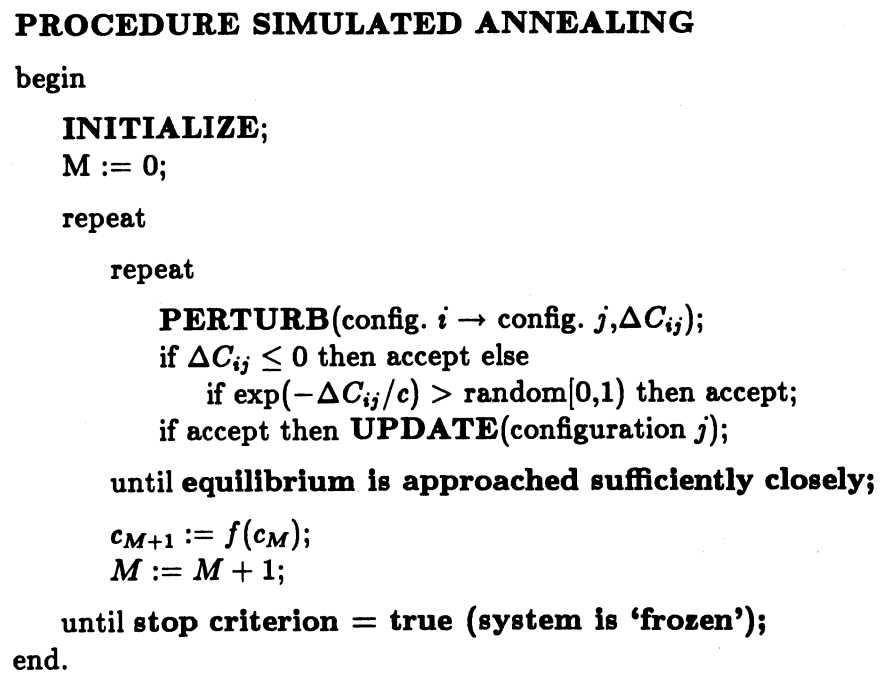
\includegraphics[width=1\textwidth]{./dados/figuras/procedure_simulated_annealing}
	\fonte{Figura 2.1 de \citeonline{van_1987}}
	\label{fig:procedure}
\end{figure}

No algoritmo \ref{alg:otimizadorInicial}, o valor da taxa de resfriamento é de 0,99, sendo a temperatura inicial e o número de passos por iteração escolhidos empiricamente. Sobre a temperatura inicial, esta deve receber um valor suficientemente alto para que possibilite as diversas trocas de posições da grade horária para a geração de uma solução satisfatória, mas não tão alto a ponto de fazer o algoritmo passar boa parte do tempo de execução realizando trocas aleatórias. Este valor 
pode ser definido empiricamente, ou utilizando o método explicitado por \citeonline{abramsomCooling}, em que é calculada a temperatura em que as soluções passam por uma transição de fase.

Explicando melhor o algoritmo, o método ``CriaGradeInicial''  gera uma matriz com as turmas e números de aulas de cada professor alocados corretamente. Esta grade inicial provavelmente possui inúmeros conflitos, portanto são aplicados os passos de otimização. Para cada passo de otimização, são escolhidas aleatoriamente uma turma e duas linhas (posições) da grade horária. Com estas informações, é calculada a variação do número de conflitos que a permutação dos professores nas linhas escolhidas ocasionaria. 

De acordo com o valor de variação calculado (delta), é determinado se a troca dos professores deve ou não ser realizada: uma troca que diminua o número de conflitos sempre é aceita, enquanto uma troca que aumenta o número de conflitos pode ser aceita probabilistacamente, de acordo com o valor da temperatura na iteração atual.

Em relação à condição de parada, durante o desenvolvimento deste primeiro incremento optou-se por utilizar o esgotamento da temperatura, ou seja, o algoritmo finaliza sua execução assim que a temperatura atinge um valor próximo de zero, quando não ocorrem mais permutações de professores.



\subsection{PESOS E RESTRIÇÕES}
\label{subsec:pesos_e_restricoes}

Apesar da importância da resolução de conflitos, existem diversas outras nuances durante o planejamento das grades horárias que precisam ser levadas em conta para que as grades produzidas sejam aplicáveis na prática.

\citeonline{ABRAMSON} sugere uma forma de permitir a otimização de múltiplas características simultanemente utilizando: uma função de custo ponderado. Esta função foi implementada, utilizando-se um sistema de métricas, cada qual mensura quantitativamente determinada característica da grade horária, e contém um peso que define a sua importância para a grade como um todo. 

A função de custo ponderado retorna um valor que representa a qualidade geral de uma grade horária, através do cálculo da média ponderada de todas as métricas de qualidade. Em outras palavras, quanto menor o custo, melhor a solução encontrada.

Adicionalmente, as métricas foram implementadas de forma que pudessem ser rígidas ou suaves. As métricas rígidas precisam ser perfeitamente atendidas para que a grade horária seja considerada viável, enquanto as métricas suaves promovem a melhoria da qualidade, mas não necessariamente precisam ser perfeitamente atendidas.

As próximas seções terão como objetivo explicar cada uma destas métricas e os desafios associados. A \autoref{subsec:salvamento} entrará em mais detalhes sobre como as grades horárias passaram a ser salvas após a implementação das métricas.

\subsubsection{Agrupamento de aulas}

Observando grades horárias escolares existentes, é possível notar que existe uma motivação para realizar agrupamentos, formando aulas duplas. Isso aumenta a produtividade das aulas, à medida que diminui trocas e deslocamento de professores entre as salas. Para produzir estes agrupamentos, foram adicionadas algumas métricas que fazem o otimizador penalizar:

\begin{enumerate}
	\item Aulas separadas;
	\item Aulas desagrupadas;
	\item Excessos de aulas iguais para determinada turma em um dia;
	\item Dias com todas aulas planejadas distintas para deteriminada turma;
\end{enumerate}

Para contextualizar estas situações, a seguir serão apresentados alguns quadros.

\begin{quadro}[!htb]
	\centering
	\caption{Exemplo de dia com aulas separadas.\label{qua:aulasSeparadas}}
	\begin{tabular}{|p{3cm}|p{3cm}|p{3cm}|}
		\hline
		\textbf{Aula} & \textbf{Professor} & \textbf{Matéria} \\
		\hline
		1 & Marcos & Matemática \\
		\hline
		2 & Fábio & Física \\
		\hline
		3 & Marcos & Matemática \\
		\hline
		4 & Luciana & Português \\
		\hline
		5 & Luciana & Português \\
		\hline
		6 & Luciana & Português \\
		\hline
	\end{tabular}
	\fonte{Autoria própria}
\end{quadro}
\pagebreak

Observando o quadro \ref{qua:aulasSeparadas}, é possível notar:

\begin{itemize}
	\item Aulas separadas: 1, 2 e 3, visto que não estão em nenhum agrupamento;
	\item Aulas desagrupadas: 1 e 3, pois consistem em múltiplas aulas iguais, no mesmo dia, que não foram agrupadas;
	\item Excessos de aulas: 4, 5, 6, pois consiste em uma aula tripla, algo considerado não desejável neste trabalho
\end{itemize}

Por fim, a situação de dias com todas aulas diferentes, que serão referidos como "Dias fragmentados" neste trabalho, pode ser observada no quadro \ref{qua:fragmentado}.

\begin{quadro}[!htb]
	\centering
	\caption{Exemplo de dia fragmentado.\label{qua:fragmentado}}
	\begin{tabular}{|p{3cm}|p{3cm}|p{3cm}|}
		\hline
		\textbf{Aula} & \textbf{Professor} & \textbf{Matéria} \\
		\hline
		1 & Marcos & Matemática \\
		\hline
		2 & Fábio & Física \\
		\hline
		3 & Luciana & Português \\
		\hline
		4 & Roberto & Geografia \\
		\hline
		5 & Renato & História \\
		\hline
	\end{tabular}
	\fonte{Autoria própria}
\end{quadro}

\subsubsection{Constantes}

Durante o desenvolvimento, concebeu-se o conceito de ``Aulas constantes'', como aulas que absolutamente devem ser alocadas em determinada posição da grade horária. Isto é útil para guiar o otimizador rumo a uma solução desejada, quando já são conhecidas algumas aulas que devem ser fixas. 

Como exemplo de caso de uso, uma escola com seis aulas diárias pode ter alguns dias da semana com menos aulas, e pode ser interessante definir explicitamente quais dias devem ter a última aula da grade horária não alocada (vazia). A figura \ref{fig:constantes} mostra um exemplo de configuração de aulas constantes para determinada grade horária.

\begin{figure}[!htb]
	\centering
	\caption{Aulas constantes}
	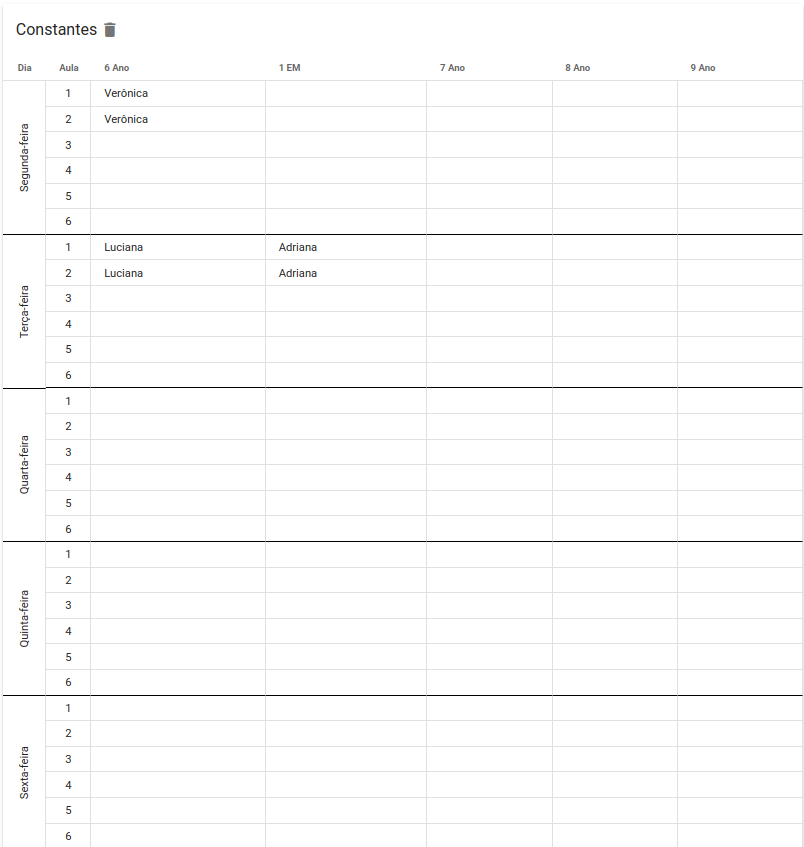
\includegraphics[width=1\textwidth]{./dados/figuras/constantes}
	\fonte{Autor}
	\label{fig:constantes}
\end{figure}
\pagebreak

Considerando a natureza absoluta das aulas constantes, estas não são consideradas um métrica de qualidade, e não possuem um peso próprio. Em vez disso, no método ``GeraGradeInicial'' do algoritmo \ref{alg:otimizadorInicial}, o otimizador já aloca as aulas constantes nas posições desejadas, e a função ``EscolheHorariosAleatoriosValidos'' não seleciona posições que estejam alocadas com aulas constantes. Desta forma, um vez que as aulas constantes são posicionadas na grade horária, estas nunca são movidas durante os passos de otimização.

\subsubsection{Restrições}

As restrições representam o oposto das aulas constantes: posições em que determinadas aulas não devem ser alocadas. Implementaram-se no otimizador restrições suaves e rígidas, cada uma podendo também receber um peso customizado. Dessa forma, é possível configurar o otimizador para nunca alocar determinada aula em certa posição da grade, ou apenas evitar isso.

Como exemplo de uso dessa funcionalidade, a figura \ref{fig:restricoes} demonstra uma configuração de restrições para determinado professor que não pode ser alocado nas duas últimas aulas de qualquer dia da grade horária.

\begin{figure}[!htb]
	\centering
	\caption{Restrições}
	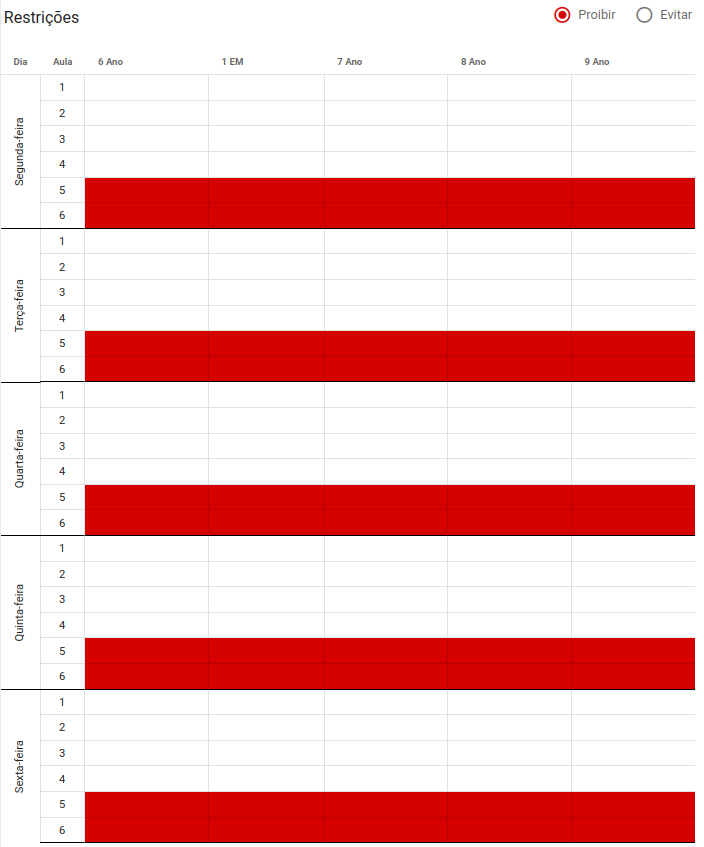
\includegraphics[width=1\textwidth]{./dados/figuras/restricoes}
	\fonte{Autor}
	\label{fig:restricoes}
\end{figure}
\pagebreak

No caso das restrições, a métrica associada mensura a quantidade de restrições violadas, ou seja, posições em que determinada aula foi alocada, mas não deveria ter sido.

\subsubsection{Regiões}

O conceito de regiões foi concebido como uma forma de proporcionar ainda mais controle ao usuário, sobre o posicionamento das aulas na grade horária. Cada região consiste em um grupo arbitrário de posições da grade horária, associado a uma regra relacionada a uma quantidade de aulas. Com as regiões, é possível determinar mínimos, máximos ou quantidades exatas de aulas que devem ser alocadas em certas posições da grade horária.

Como exemplo de uso das regiões, a figura \ref{fig:regioes} demonstra uma configuração utilizada para assegurar que em todos os dias da grade horária, o professor tenha alguma aula alocada no primeiro horário.

\begin{figure}[!htb]
	\centering
	\caption{Exemplo de região}
	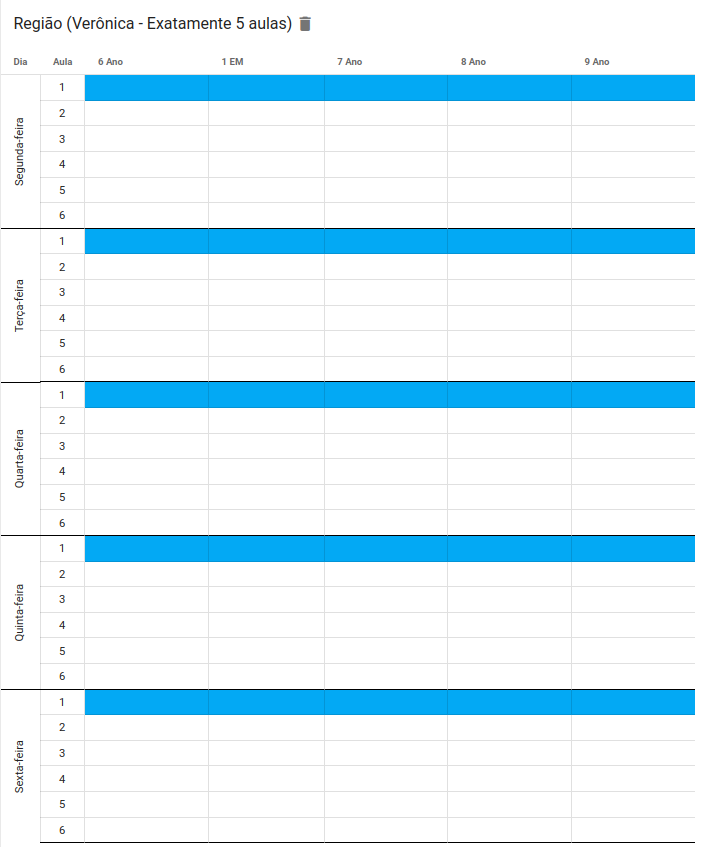
\includegraphics[width=1\textwidth]{./dados/figuras/regioes}
	\fonte{Autor}
	\label{fig:regioes}
\end{figure}
\pagebreak

A região configurada na \ref{fig:regioes} pode ser interpretada da seguinte forma: a professora ``Verônica'' deve ter exatamente cinco aulas alocadas dentro das posições marcadas pela cor azul. Como o otimizador não permite conflitos, cada uma das cinco aulas deverá ser alocada em um dos diferentes dias, garantindo que a professora terá uma aula agendada no primeiro horário de cada um dos dias.

Neste caso, a métrica associada mensura o erro das regiões, ou seja, a diferença entre a quantidade de aulas esperada de acordo com a regra de cada região e a quantidade real de aulas alocadas.

\subsubsection{Grupos de Alinhamento}

Os grupos de alinhamento representam uma forma de configurar o otimizador para agendar aulas para diferentes turmas, nos mesmos horários. Isto é útil para atender a restrições relacionadas ao conceito dos Itinrários Formativos do Novo Ensino Médio, conforme citado na \autoref{sec:novo_ensino_medio}.

Como exemplo de utilização dos grupos de alinhamentos, tem-se a configuração da figura \ref{fig:gruposAlinhamento}.

\begin{figure}[!htb]
	\centering
	\caption{Exemplo de grupo de alinhamento sobre a grade horária gerada}
	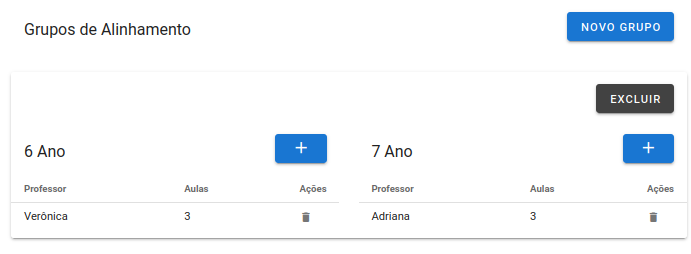
\includegraphics[width=1\textwidth]{./dados/figuras/gruposAlinhamento}
	\fonte{Autor}
	\label{fig:gruposAlinhamento}
\end{figure}
\pagebreak

O efeito da configuração do grupo de alinhamento da figura \ref{fig:gruposAlinhamento}, pode ser observado na grade horária final gerada na figura \ref{fig:alinhados}, com as aulas corretamente alocadas em horários simultâneos.

\begin{figure}[!htb]
	\centering
	\caption{Efeito de grupo de alinhamento}
	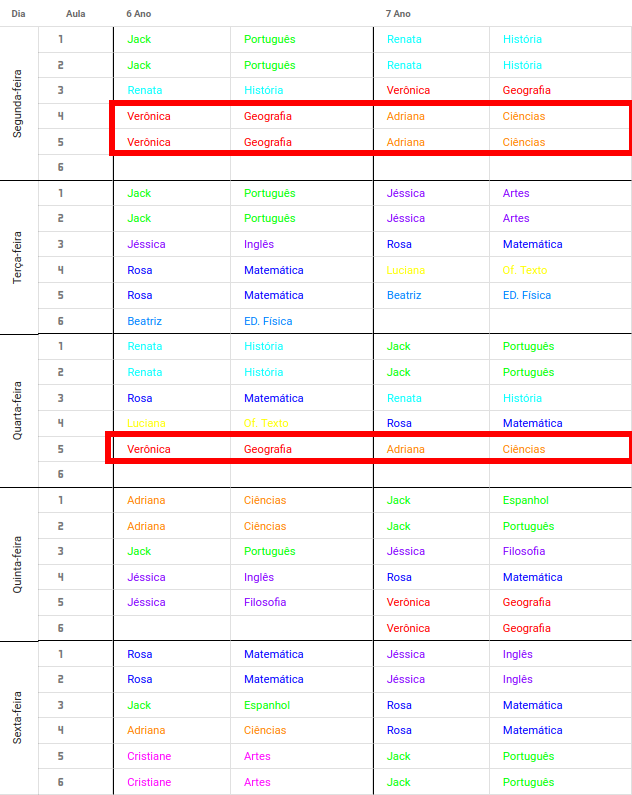
\includegraphics[width=1\textwidth]{./dados/figuras/alinhados}
	\fonte{Autor}
	\label{fig:alinhados}
\end{figure}
\pagebreak

Implementaram-se duas métricas de qualidade relacionadas aos grupos de alinhamento, uma que mensura a quantidade de grupos formados e a quantidade de aulas ``desalinhadas'', ou seja, aulas que deveriam ser agendadas no mesmo horário, mas que não foram.

No caso da \ref{fig:alinhados}, foram formados dois grupos (demarcados em vermelho), e nenhuma aula ficou desalinhada, ou seja, todas as seis aulas configuradas no grupo de alinhamento foram corretamente alocadas em horários simultâneos.

\subsubsection{Janelas}

As janelas consistem em situações em que a jornada de trabalho de determinado professor apresenta um horário sem aulas alocadas, fazendo com que o docente fique ocioso. O quadro \ref{qua:janelas} exemplifica esta situação.

\begin{quadro}[!htb]
	\centering
	\caption{Exemplo de dia com janela.\label{qua:janelas}}
	\begin{tabular}{|p{3cm}|p{3cm}|p{3cm}|p{3cm}|}
		\hline
		\textbf{Aula} & \textbf{6ºAno} & \textbf{7ºAno} & \textbf{8ºAno} \\
		\hline
		1 & Jéssica & Rosa & Adriana \\
		\hline
		2 & Jéssica & Rosa & Adriana \\
		\hline
		3 & Fábio & Jéssica & Rosa \\
		\hline
		4 & Adriana & Jéssica & Rosa \\
		\hline
		5 & Beatriz & Adriana & Jéssica \\
		\hline
	\end{tabular}
	\fonte{Autoria própria}
\end{quadro}

No quadro \ref{qua:janelas}, a professora Adriana tem uma janela na terceira aula, visto que tem aulas alocadas antes e depois (aulas 1, 2, 4 e 5). Em contrapartida, apesar de não ter nenhuma aula planejada no quinto horário, Rosa não tem janelas neste exemplo, pois pode encerrar sua jornada de trabalho na quarta aula.

A métrica de janelas mensura o número de horários na grade que apresentam estes horários ociosos, para cada professor.

\subsubsection{Preferências}

As preferências consistem em configurações que informam ao otimizador características preferíveis para a alocação das aulas de cada professor. Implementaram-se os seguintes tipos de preferência no otimizador:

\begin{enumerate}
	\item Preferência de primeiras aulas;
	\item Preferência de últimas aulas;
	\item Preferência específica de última aula
\end{enumerate}

\begin{figure}[!htb]
	\centering
	\caption{Configuração de preferências}
	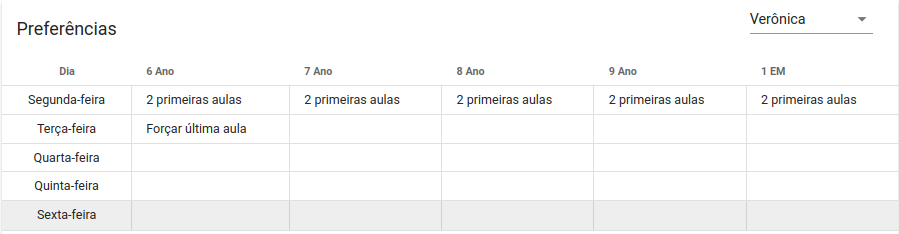
\includegraphics[width=1\textwidth]{./dados/figuras/preferencias}
	\fonte{Autor}
	\label{fig:preferencias}
\end{figure}

A \autoref{fig:preferencias} representa um exemplo de configuração de preferências para determinado professor. Neste caso, a configuração informa ao otimizador que na segunda-feira, as aulas de ``Verônica'' devem ser alocadas desde o início do dia, não ultrapassando um total de aulas; e que na turma do ``6º Ano'', caso haja uma aula dessa professora, esta deve ser alocada na última aula.

Vale ressaltar que o diferencial da preferência específica de última aula é que esta considera a possibilidade de aulas vazias, ou seja, caso o último horário do dia não tenha uma aula alocada, a preferência considera que a aula deve ser alocada na penúltima aula.

\subsubsection{Mínimos e máximos}

Desenvolveram-se métricas de qualidade relacionadas a quantidades de aulas ministradas por dia. Como pode ser visto na figura \ref{fig:tela_minimos}, estas métricas permitem configurar quantidades mínimas e máximas de aulas por dia para cada professor.

\begin{figure}[htb!]
	\centering
	\caption{Mínimos de aulas configuradas na interface}
	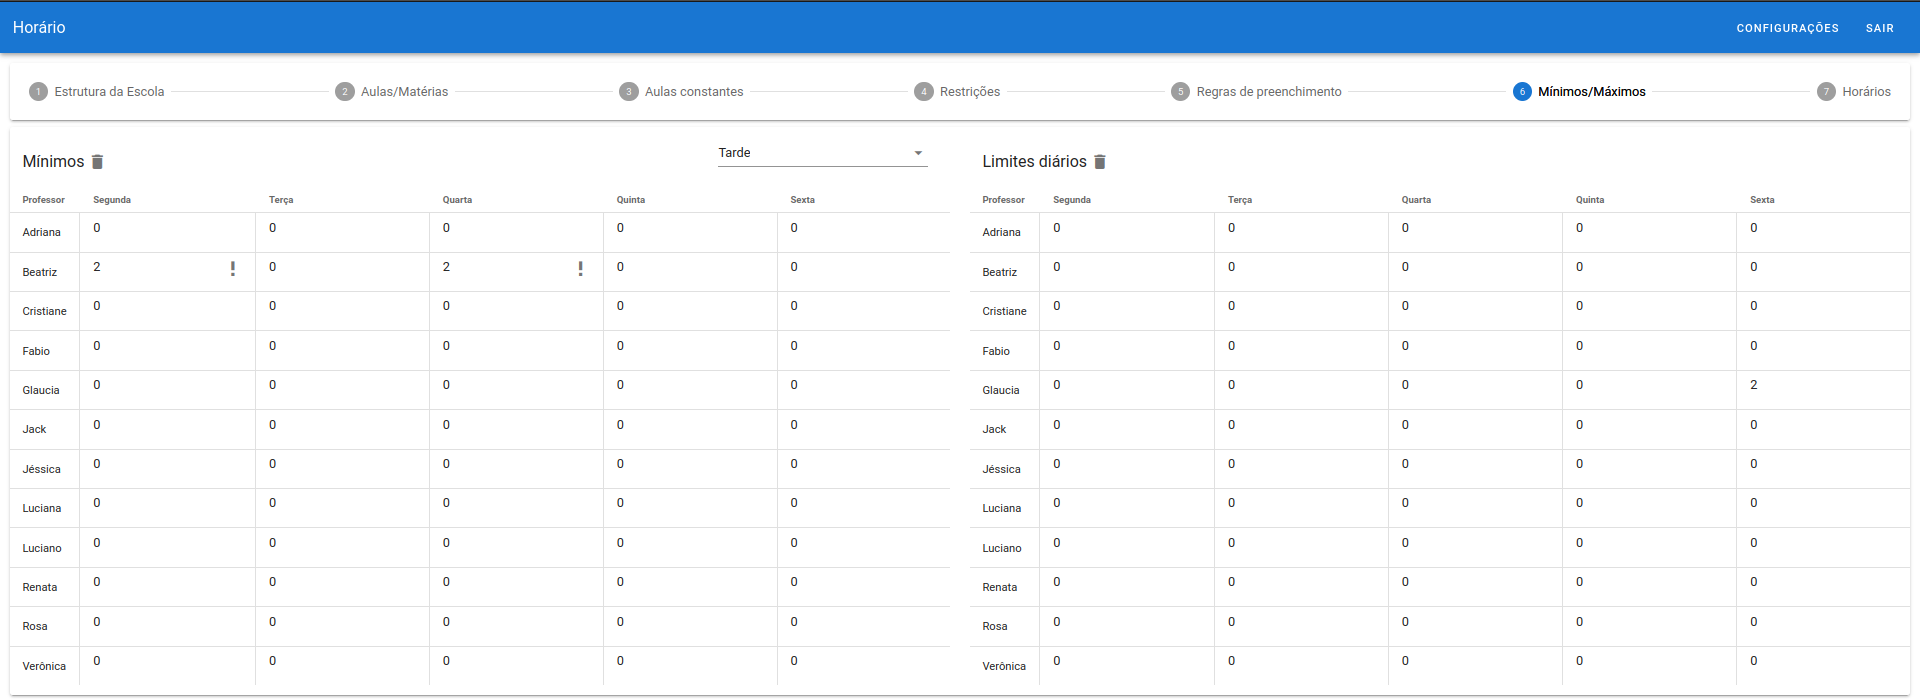
\includegraphics[width=1\textwidth]{./dados/figuras/minimos_configurados}
	\fonte{Autor}
	\label{fig:tela_minimos}
\end{figure}

O cálculo das métricas de qualidade relacionadas aos mínimos e máximos consiste no cálculo do erro, ou seja a quantidade de aulas alocada subtraída da quantidade de aulas esperada. Vale ressaltar que enquanto os mínimos são configuráveis por turno, os máximos são interpretados como limites diários, e consequentemente levam em conta a soma da quantidade de aulas em todos os turnos. Por exemplo, se um professor tem um limite diário de cinco aulas configurado, a soma de suas aulas naquele dia, em todos os turnos, não deverá ultrapassar cinco.

\subsubsection{Armazenamento de soluções}
\label{subsec:salvamento}

Com a adição das métricas, o critério para considerar uma grade horária como uma solução válida ficou mais estrito, e em muitos casos tornou-se impossível obter uma grade que atenda perfeitamente todas as nuances. Tendo isto em mente, foi necessário implementar uma funciondalide de armazenamento de grades horárias um pouco mais detalhada. O resultado disso, pode ser visto no algoritmo \ref{alg:otimizadorComRestricoes}.

\begin{algorithm}
	\caption{Otimizador com persistência de grades horárias}
	\label{alg:otimizadorComRestricoes}
	\KwIn{Lista de professores $LP$, lista de turmas $LT$, matriz de aulas por professor por turma $MA$, temperatura inicial $TI$, Taxa de resfriamento $TR$}
	\KwOut{Grade horária de professores otimizada}
	$temperatura \leftarrow TI$\\
	$grade \leftarrow$ CriaGradeInicial$(LP, LT, MA)$\\
	$iteracoesSemAlteracao \leftarrow 0$\\
	$solucoes \leftarrow$ lista vazia\\
	\While {condição de parada não atingida} {
		$deltaTotal \leftarrow 0$\\
		\For {$passo = 0$ até $numeroPassos$} {
			$turma \leftarrow grade.EscolheTurmaAleatoria()$\\
			$linhas \leftarrow grade.EscolheHorariosAleatoriosValidos(sala)$\\
			$delta \leftarrow grade.CalculaDelta(sala, linhas)$\\
			$probabilidade \leftarrow e^{-delta/temperatura}$\\
			$valorAceite \leftarrow Aleatorio(0, 1)$\\
			\If {$delta < 0$ ou $probabilidade \ge valorAceite$} {
				$grade.PermutaProfessores(sala, linha1, linha2)$\\
				$deltaTotal \leftarrow deltaTotal + delta$\\
				\If {grade não existe na lista de soluções} {
					insere grade na lista de soluções\\
					limita lista de soluções às 100 melhores grades\\
				}
			}
		}
		\eIf {$delta = 0$} {
			$iteracoesSemAlteracao \leftarrow iteracoesSemAlteracao + 1$\\
		}{
			$iteracoesSemAlteracao \leftarrow 0$\\
		}
		\If {$iteracoesSemAlteracao \ge 15$} {
			salvaGradesRelevantes()\\
			apaga lista de soluções\\
			$temperatura \leftarrow TI$\\
			$iteracoesSemAlteracao \leftarrow 0$\\
		}
		$temperatura \leftarrow temperatura * TR$
	}
\end{algorithm}
\pagebreak

Consinderando as diversas métricas de qualidade que as grades horárias passaram a ter, o método ``salvaGradesRelevantes'' do algoritmo \ref{alg:otimizadorComRestricoes} salva, para cada métrica escolhida, as 5 grades que tiveram a melhor pontuação em cada métrica. A princípio, optou-se por utilizar as métricas de qualidade geral (média ponderada de todas as métricas), janelas, agrupamento de aulas e número de preferências resolvidas, mas este método pode ser expandido para qualquer uma das métricas implementadas no sistema.


\section{SERVIDOR E BANCO DE DADOS}

A aplicação do lado do servidor é responsável por receber as requisições da interface, persistir as configurações no banco de dados e realizar a comunicação com o otimizador, a fim de produzir e armazenar as grades horárias.

Para o desenvolvimento deste componente, optou-se pelo \textit{framework Express.js}, a ser executado na plataforma \textit{Node.js}, devido à simplicidade de implementação que estas tecnologias proporcionam. Em relação ao banco de dados, será utilizado o sistema de gerenciamento de banco de dados \textit{PostgresSQL}, devido à sua robustez.

Conforme as premissas do problema sendo tratado, a modelagem do banco de dados é centrada na entidade ``Configuração'', que agrupa as configurações de determinada instituição de ensino para a geração de suas grades horárias. Cada uma dessas entidades tem turnos, salas, professores, e as configurações de quantas aulas cada professor deve ministrar em cada sala, e as respectivas restrições.

A modelagem comentada está representada na \autoref{fig:diagramaEr}:

\begin{figure}[!htb]
	\centering
	\caption{Modelo Entidade-Relacionamento}
	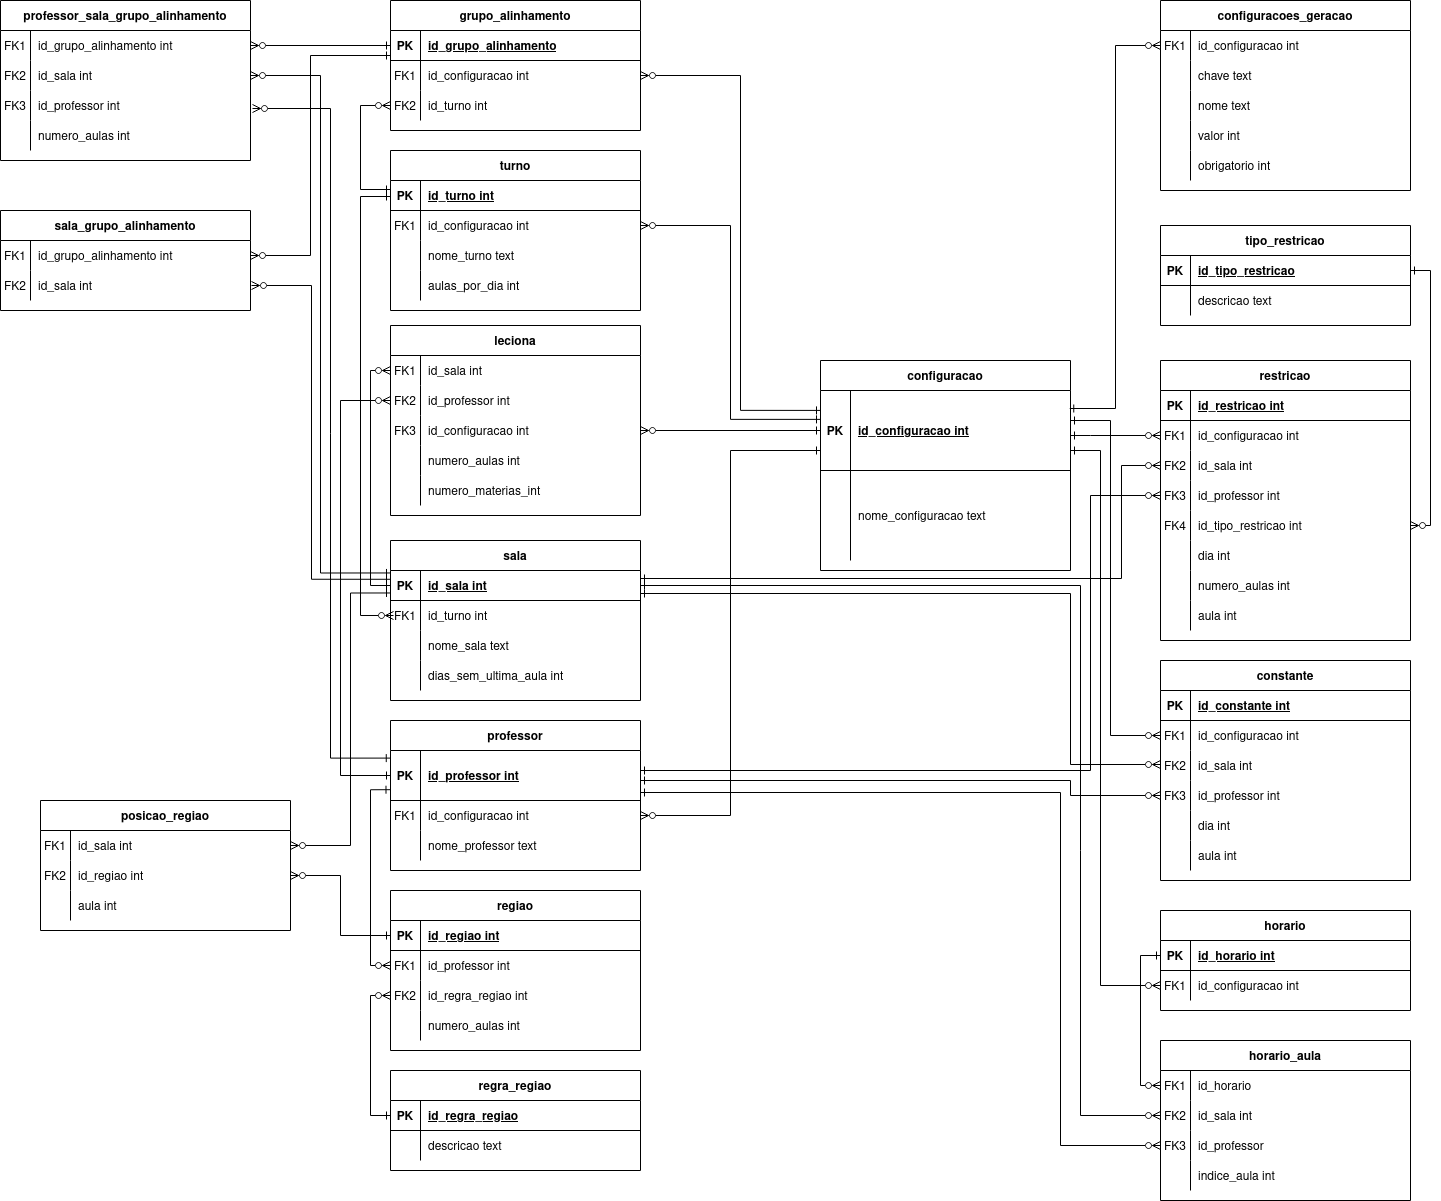
\includegraphics[width=1\textwidth]{./dados/figuras/diagrama_er}
	\fonte{Autor}
	\label{fig:diagramaEr}
\end{figure}
\newpage

Dentre as entidades mostradas no modelo entidade-relacionamento, vale ressaltar a importância da entidade ``Grupo Alinhamento''. Esta será utilizada para configurar aulas que devam acontecer simultaneamente, a fim de resolver o desafio dos itinerários formativos do Novo Ensino Médio, conforme exposto na seção \ref{sec:novo_ensino_medio}.

Para validar a modelagem do banco de dados, realizaram-se inserções de informações de exemplo nas diferentes tabelas. A \autoref{fig:sqlValidacao} mostra algumas dessas inserções e os vínculos instituídos pelos identificadores escolhidos.

\begin{figure}[!htb]
	\centering
	\caption{Consultas de validação da modelagem}
	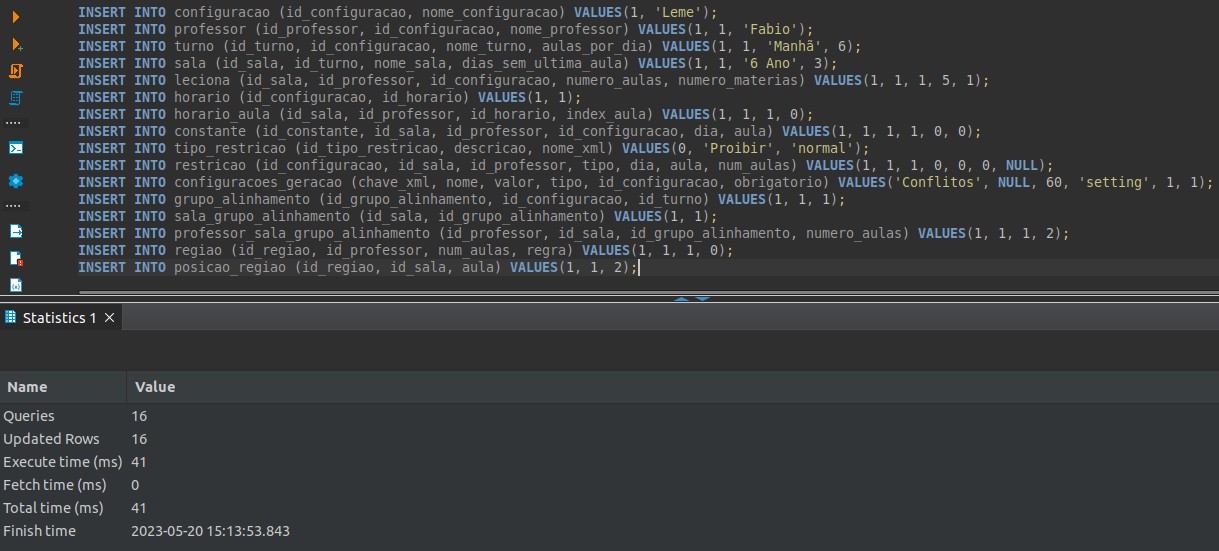
\includegraphics[width=1\textwidth]{./dados/figuras/sql_validacao}
	\fonte{Autor}
	\label{fig:sqlValidacao}
\end{figure}
\newpage

Validou-se também o armazenamento das grades horárias no banco de dados. A \autoref{fig:sqlGrade} traz um exemplo de consulta de uma grade horária com sete salas:

\begin{figure}[!htb]
	\centering
	\caption{Consulta SQL de grade horária com sete salas}
	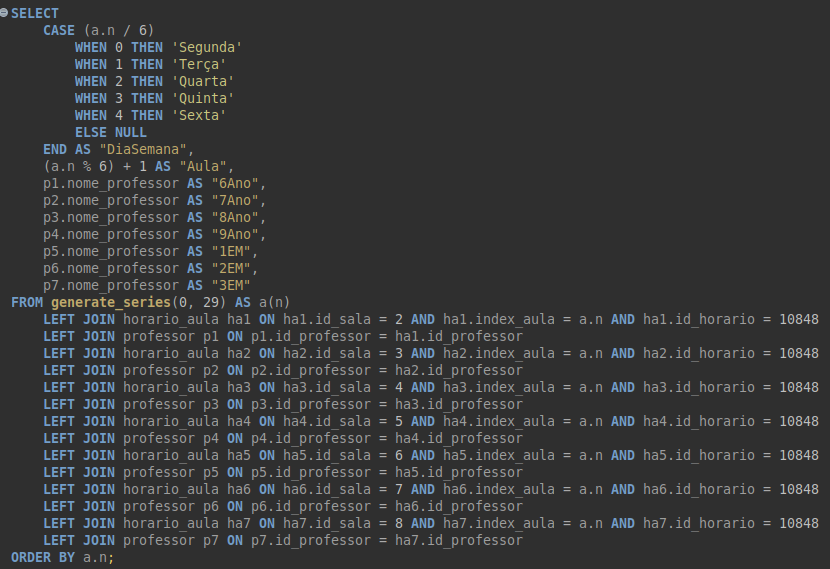
\includegraphics[width=0.7\textwidth]{./dados/figuras/sql_grade}
	\fonte{Autor}
	\label{fig:sqlGrade}
\end{figure}

A consulta anterior traz como resultado a tabela visível na \autoref{fig:consultaGrade}, com linhas e colunas correpondentes a horários de aulas e salas respectivamente.

\begin{figure}[!htb]
	\centering
	\caption{Resultado da consulta de uma grade no banco de dados}
	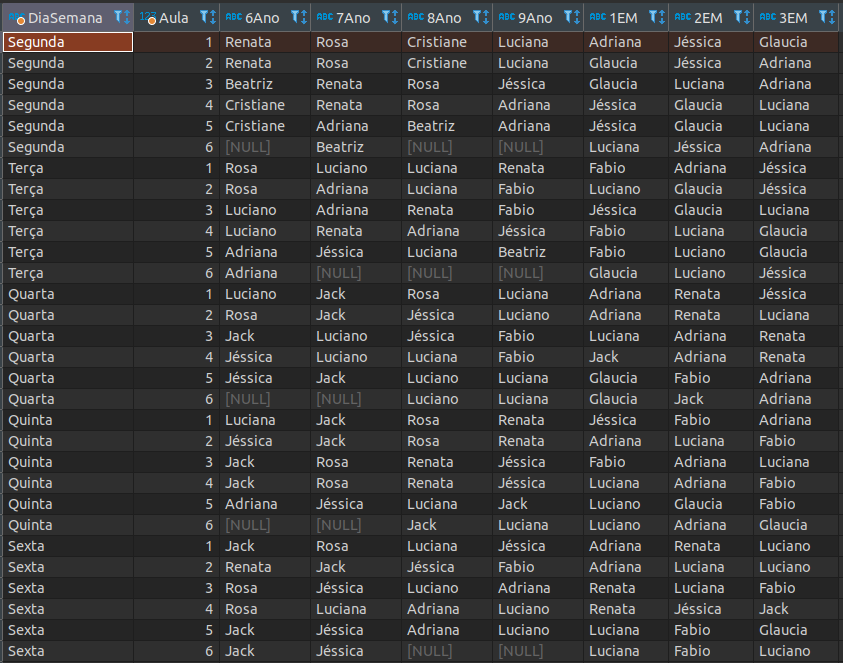
\includegraphics[width=0.7\textwidth]{./dados/figuras/ConsultaGrade}
	\fonte{Autor}
	\label{fig:consultaGrade}
\end{figure}
\section{INTERFACE}

A interface \textit{web} será responsável pela interação do usuário final com a aplicação. Portanto, deverá implementar funcionalidades que possibilitem a configuração das restrições e características das grades horárias a serem geradas, além de mostrar ou exportar tais grades após a geração.

Para o desenvolvimento deste componente, optou-se pelo framework \textit{Vue.js}, devido à riqueza de seu ecossistema de desenvolvimento \textit{frontend} e familiaridade do graduando com este. Complementando este framework, será utilizado também o \textit{Vuetify.js}, a fim de facilitar e padronizar o design da aplicação.

A \autoref{fig:diagrama-uc} mostra os casos de uso que a interface \textit{web} será responsável por disponibilizar:

\begin{figure}[!htb]
	\centering
	\caption{Diagrama de Casos de Uso}
	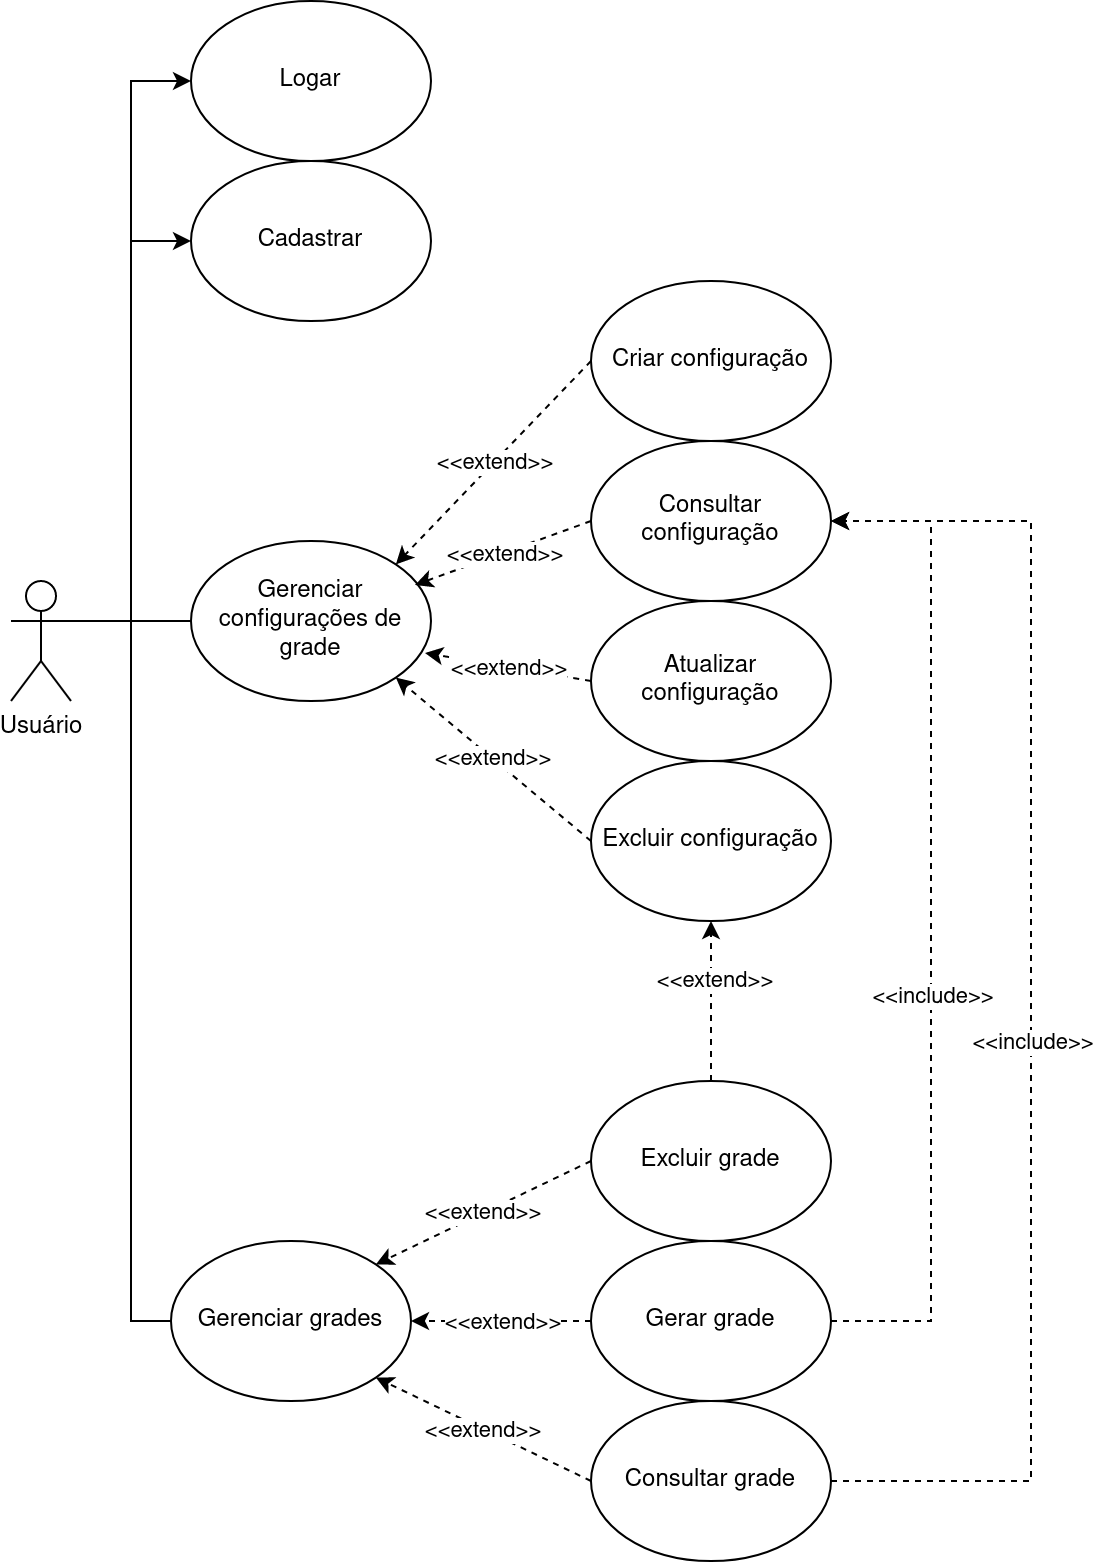
\includegraphics[width=0.65\textwidth]{./dados/figuras/diagrama_uc}
	\fonte{Autor}
	\label{fig:diagrama-uc}
\end{figure}
\newpage

Desenvolveram-se alguns protótipos iniciais das telas necessárias na aplicação.
Primeiramente, a \autoref{fig:tela-configuracoes} mostra a tela de listagem de configurações de grade. Como comentado anteriormente, alguns dos casos de uso da aplicação envolvem o gerenciamento de configurações de grades horárias, as quais são listadas nessa tela.

\begin{figure}[!htb]
	\centering
	\caption{Tela - Listagem de Configurações de Grade}
	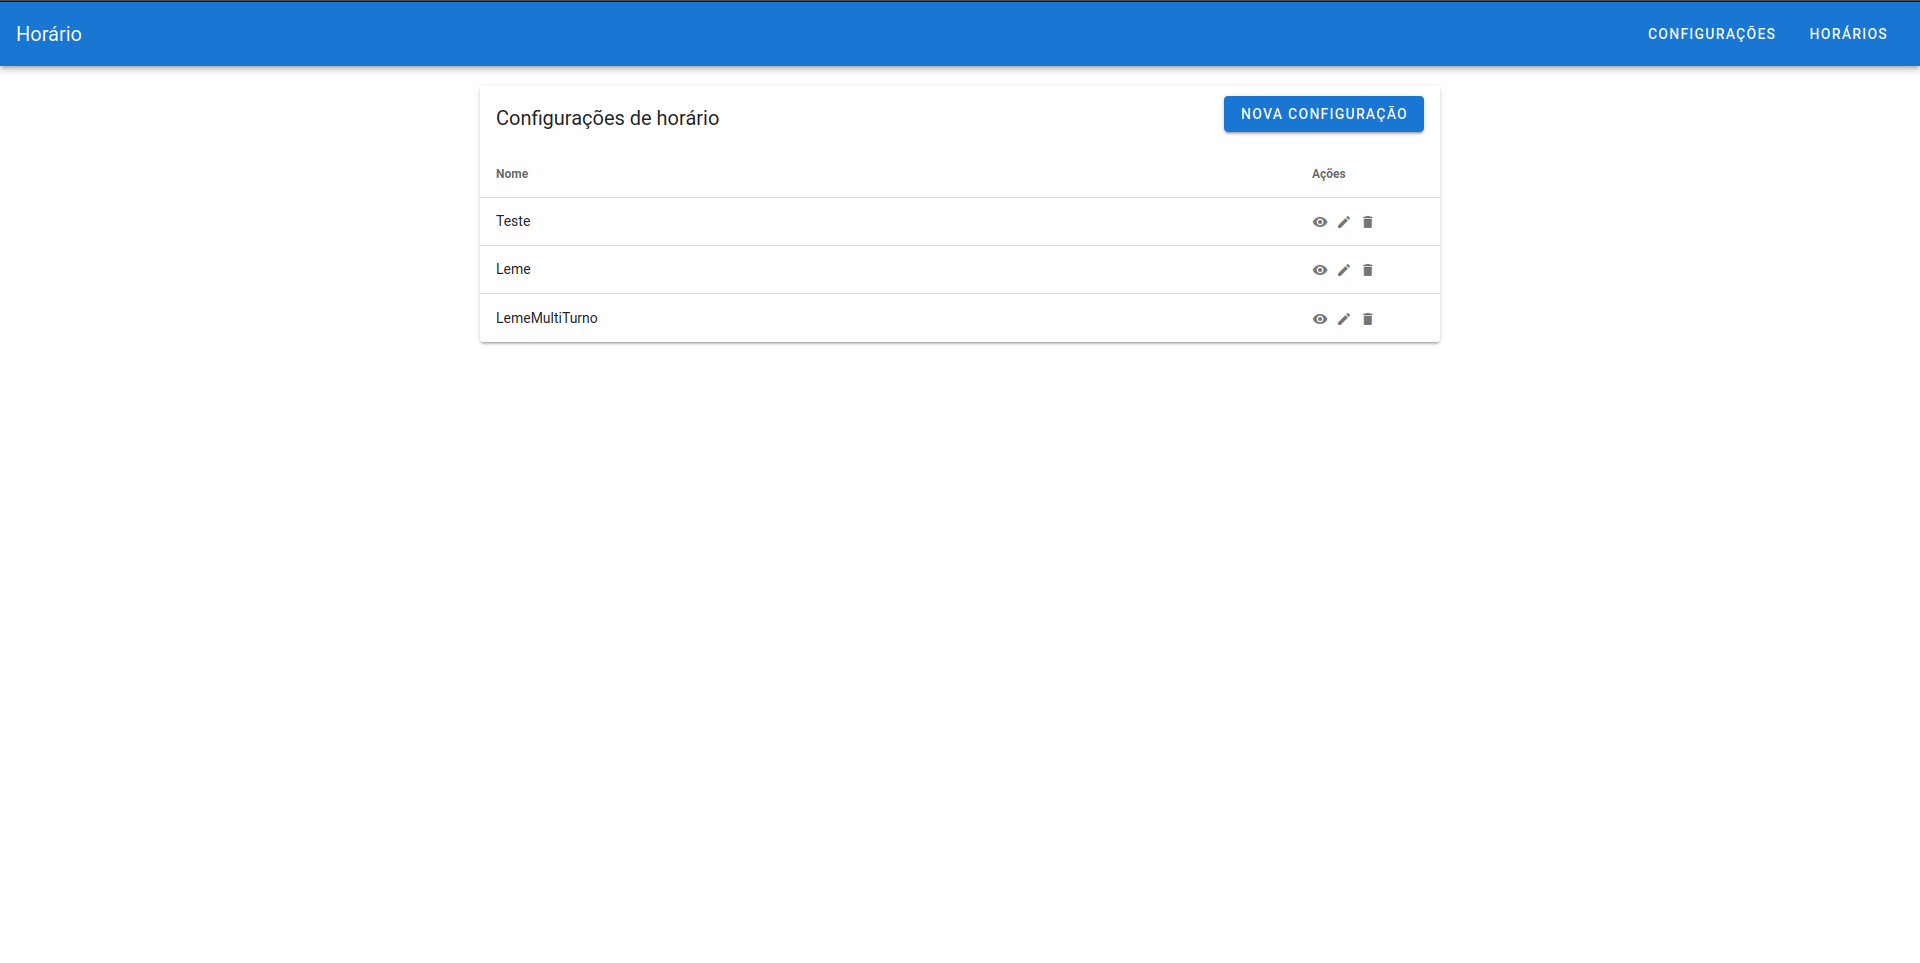
\includegraphics[width=0.8\textwidth]{./dados/figuras/tela_configuracoes}
	\fonte{Autor}
	\label{fig:tela-configuracoes}
\end{figure}
\pagebreak

A tela mostrada na \autoref{fig:tela-estrutura1} é responsável por permitir que o usuário cadastre os professores da escola. Nessa tela é possível notar que a aplicação foi estruturada seguindo uma noção de etapas de configuração até a geração da grade horária final. No topo da tela, a etapa "Estrutura da Escola" encontra-se selecionada.

\begin{figure}[!htb]
	\centering
	\caption{Tela - Estrutura da Escola - Professores}
	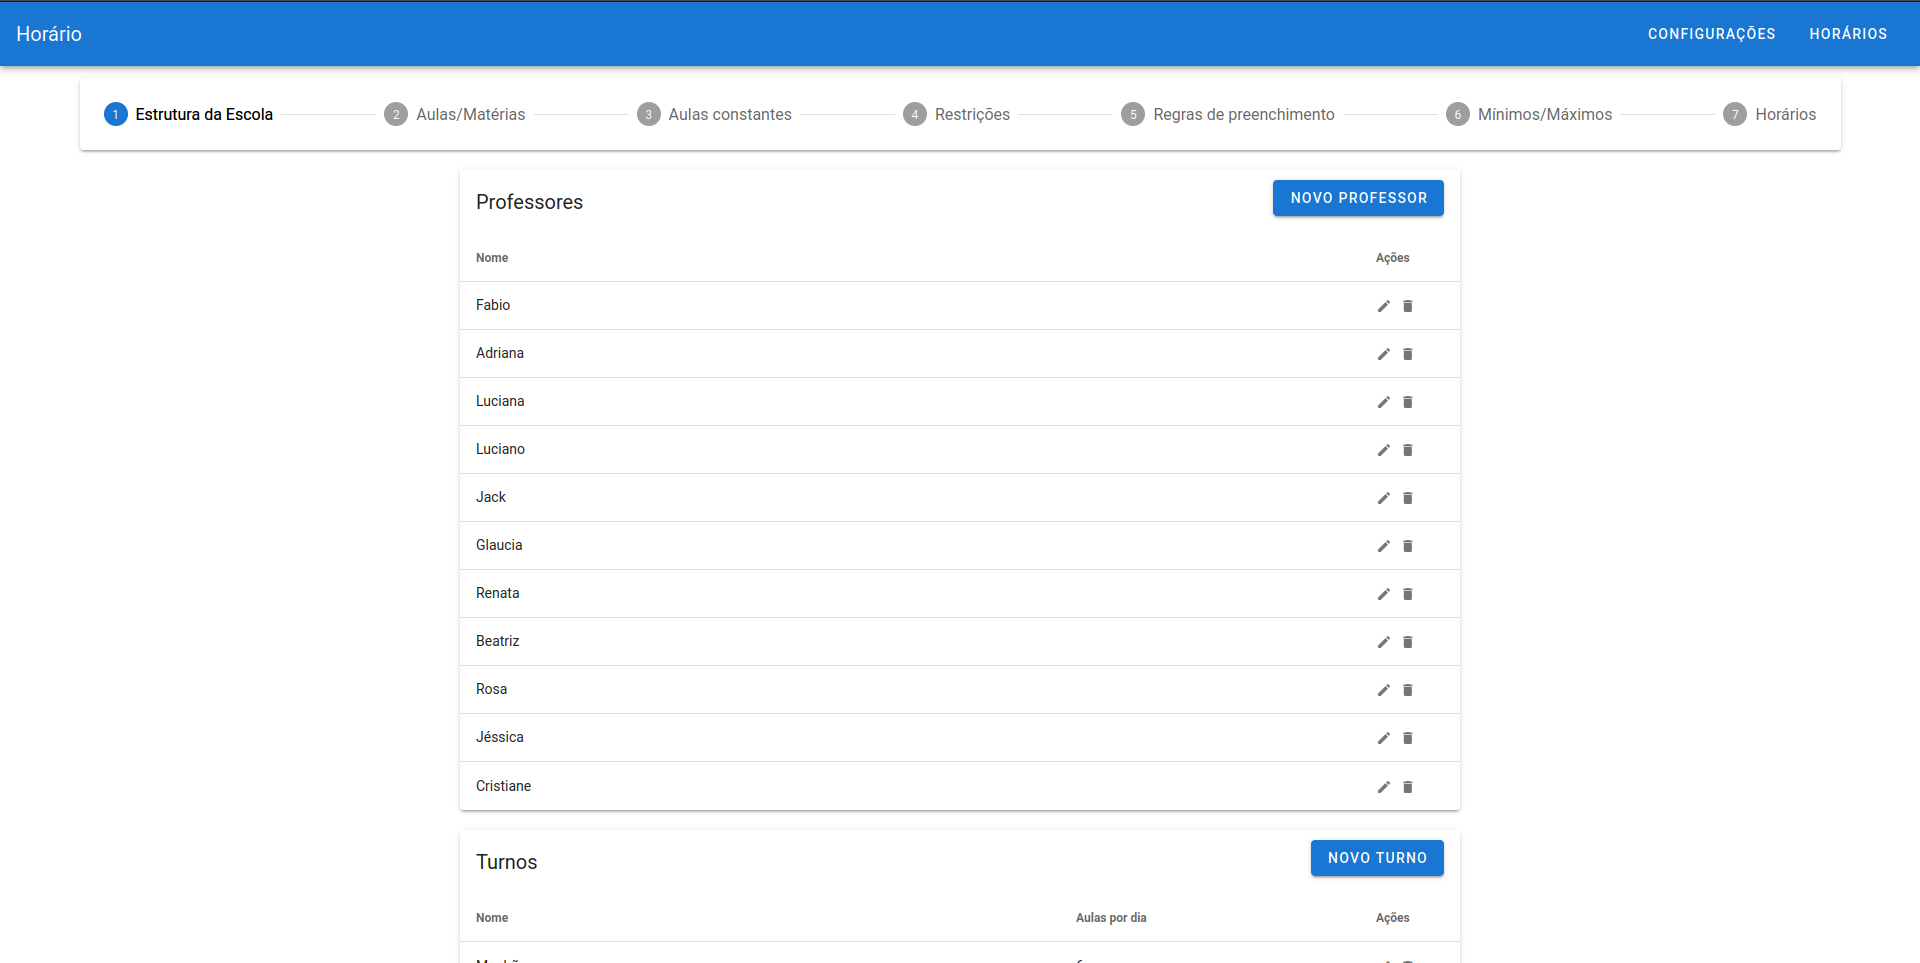
\includegraphics[width=0.8\textwidth]{./dados/figuras/tela_estrutura1}
	\fonte{Autor}
	\label{fig:tela-estrutura1}
\end{figure}
\newpage

Na \autoref{fig:tela-estrutura2}, tem-se a continuação da tela de estrutura da escola, mostrada na \autoref{fig:tela-estrutura1}. Esta parte da tela é responsável pela configuração das salas e turnos da escola.

\begin{figure}[!htb]
	\centering
	\caption{Tela - Estrutura da Escola - Salas e Turnos}
	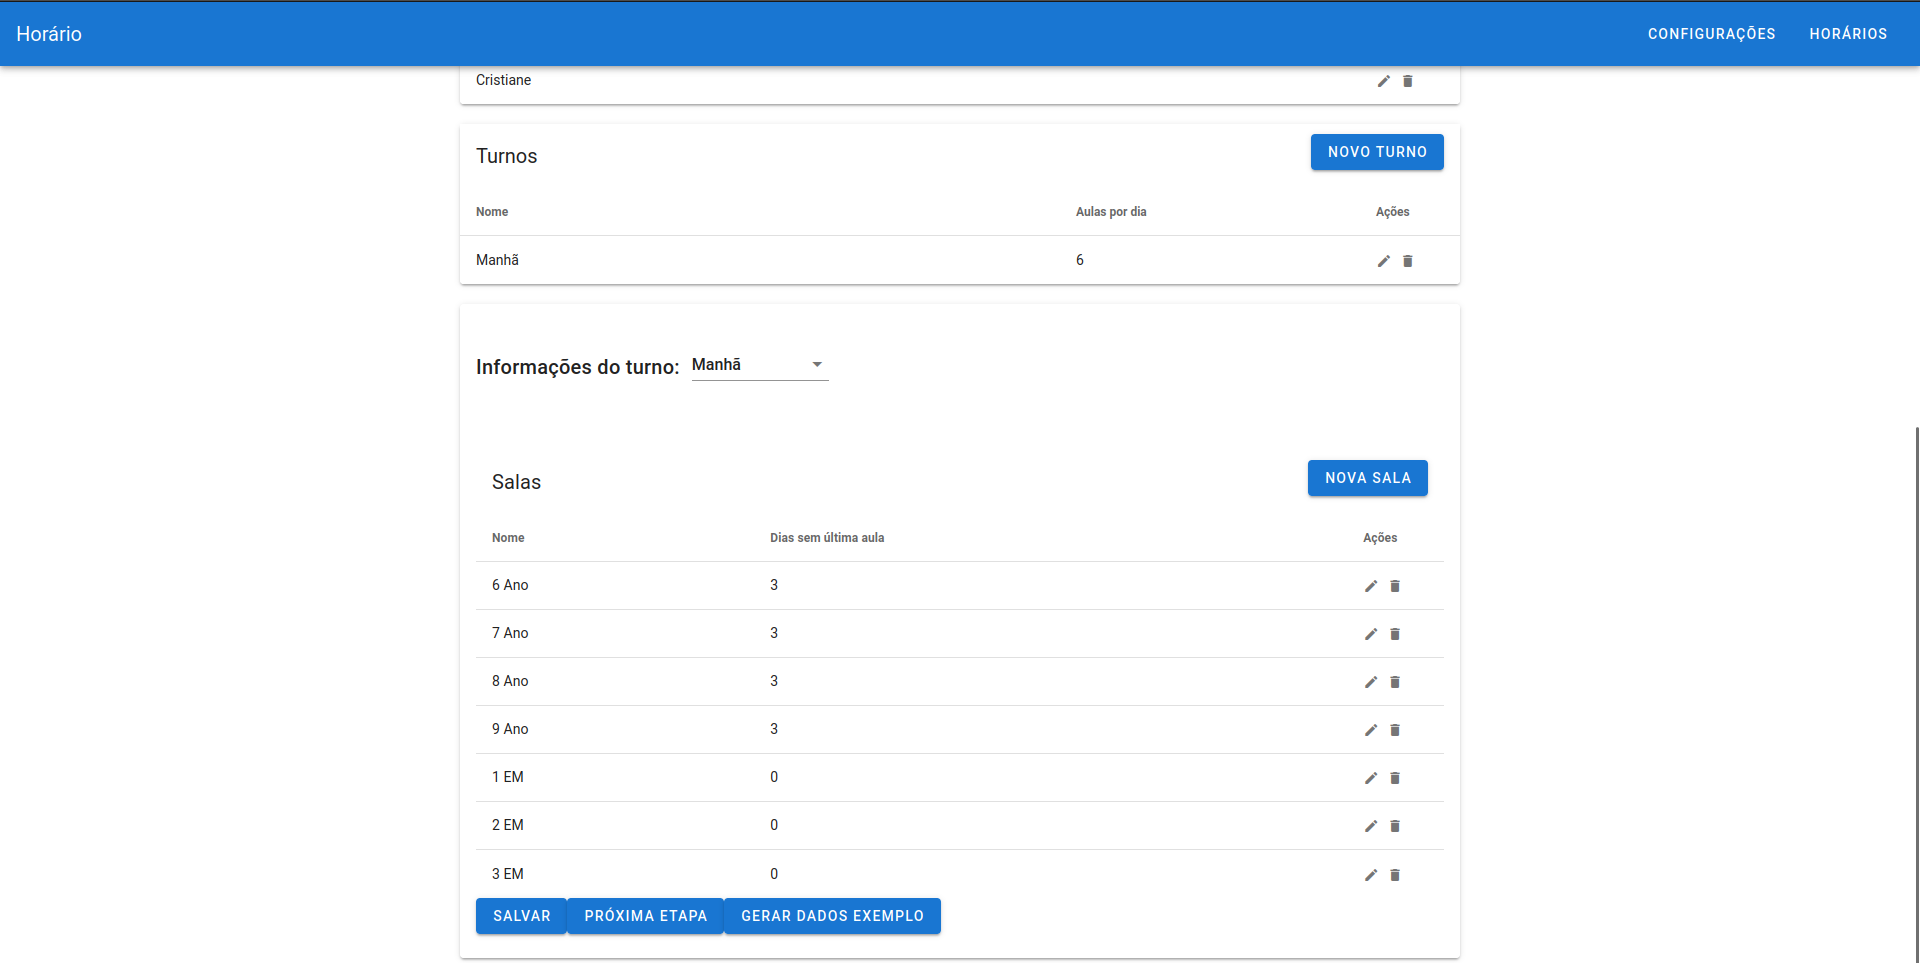
\includegraphics[width=0.8\textwidth]{./dados/figuras/tela_estrutura2}
	\fonte{Autor}
	\label{fig:tela-estrutura2}
\end{figure}

Na tela da \autoref{fig:tela-aulas}, o usuário pode realizar a configuração de número de aulas que cada professor deve ministrar em cada sala, informação fundamental para a geração das grades horárias.

\begin{figure}[!htb]
	\centering
	\caption{Tela - Aulas por professor}
	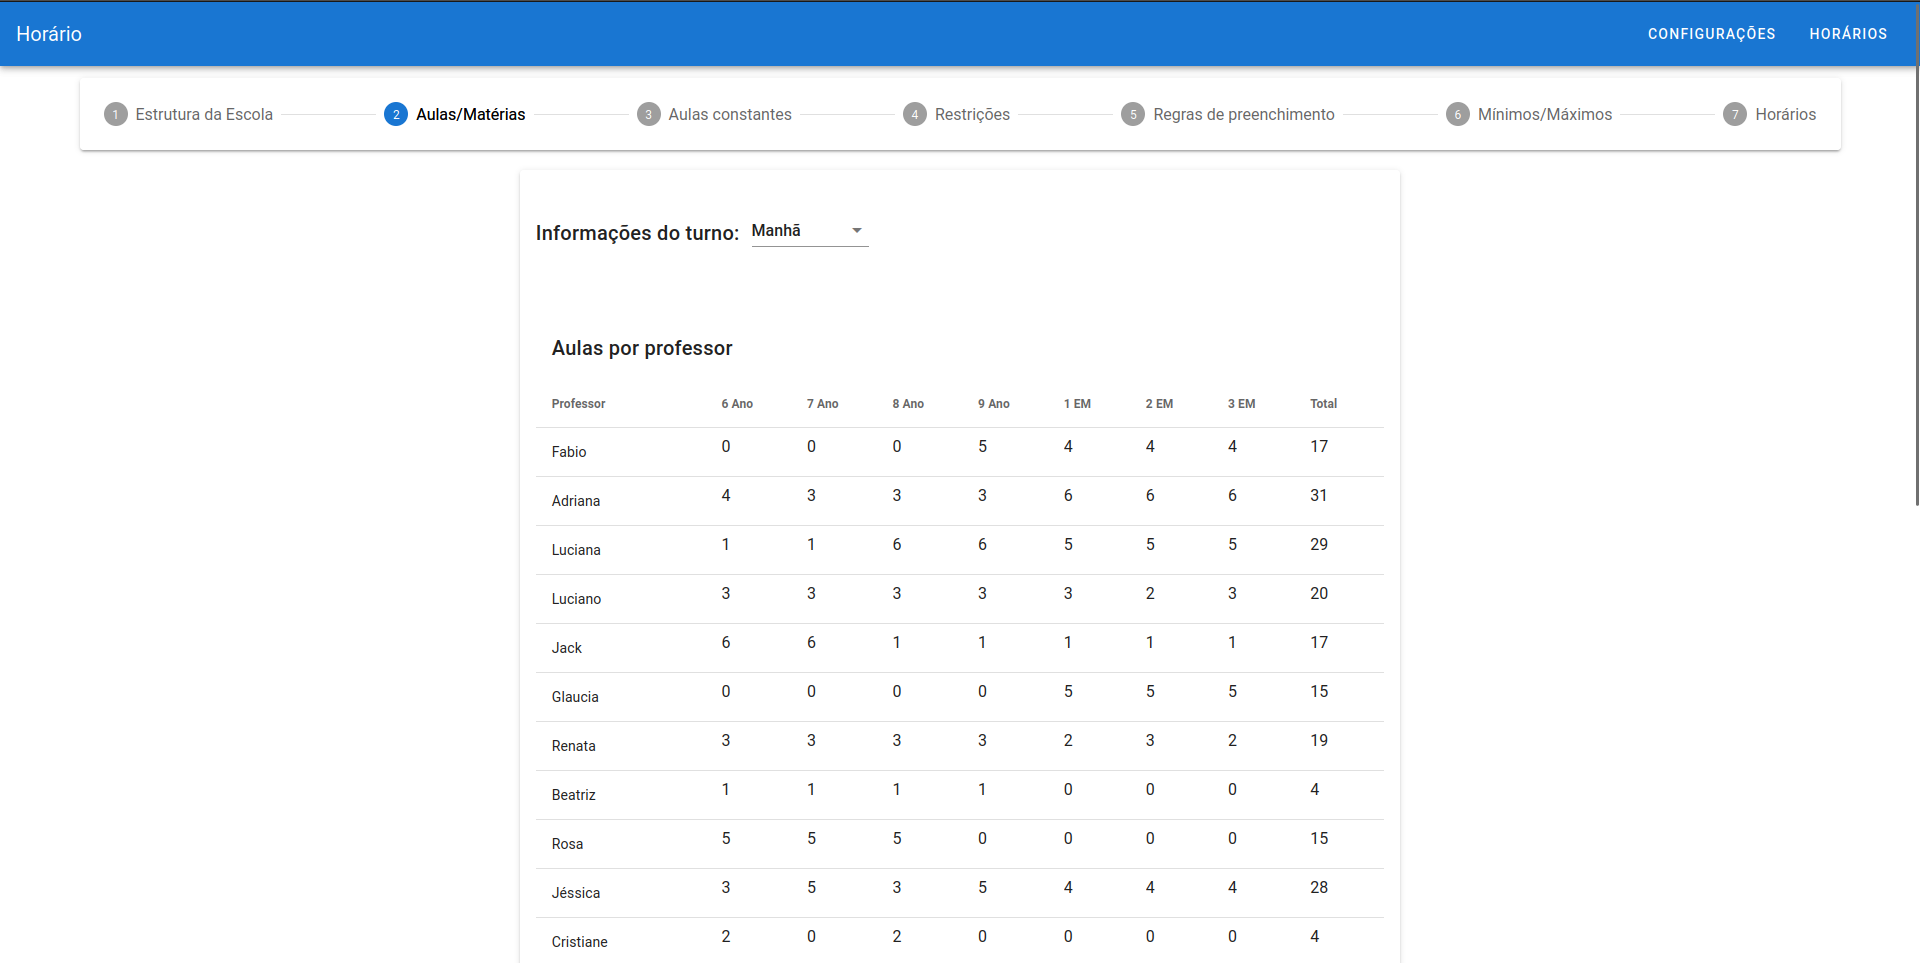
\includegraphics[width=0.8\textwidth]{./dados/figuras/tela_aulas}
	\fonte{Autor}
	\label{fig:tela-aulas}
\end{figure}
\newpage

A tela da \autoref{fig:tela-restricoes} é responsável pela configuração das restrições. Nesta, o usuário pode configurar horários na grade que devem ser evitados ou proibidos para determinado docente.

\begin{figure}[!htb]
	\centering
	\caption{Tela - Restrições}
	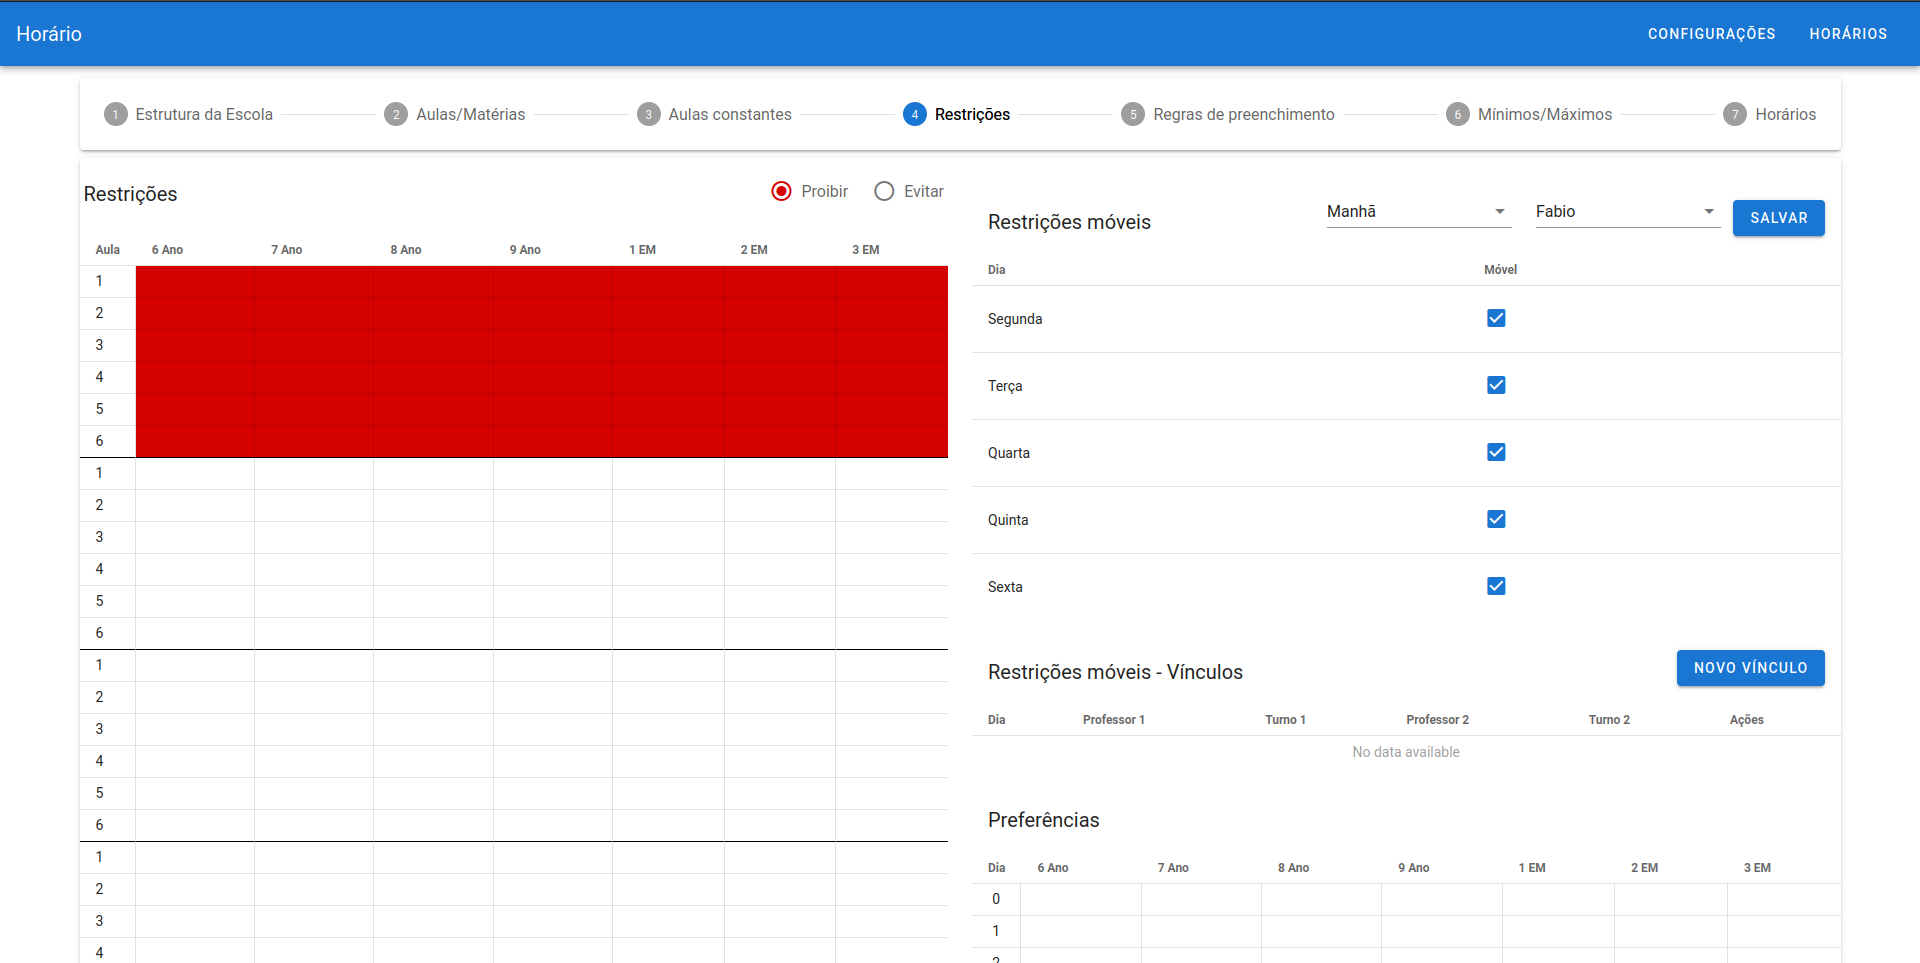
\includegraphics[width=0.8\textwidth]{./dados/figuras/tela_restricoes}
	\fonte{Autor}
	\label{fig:tela-restricoes}
\end{figure}

A última etapa no fluxo da aplicação é representada pela tela da \autoref{fig:tela-horarios}. Nesta, o usuário pode requisitar a geração da grade horária utilizando as configurações realizadas nas etapas anteriores, e acessar as grades geradas anteriormente.

\begin{figure}[!htb]
	\centering
	\caption{Tela - Horários}
	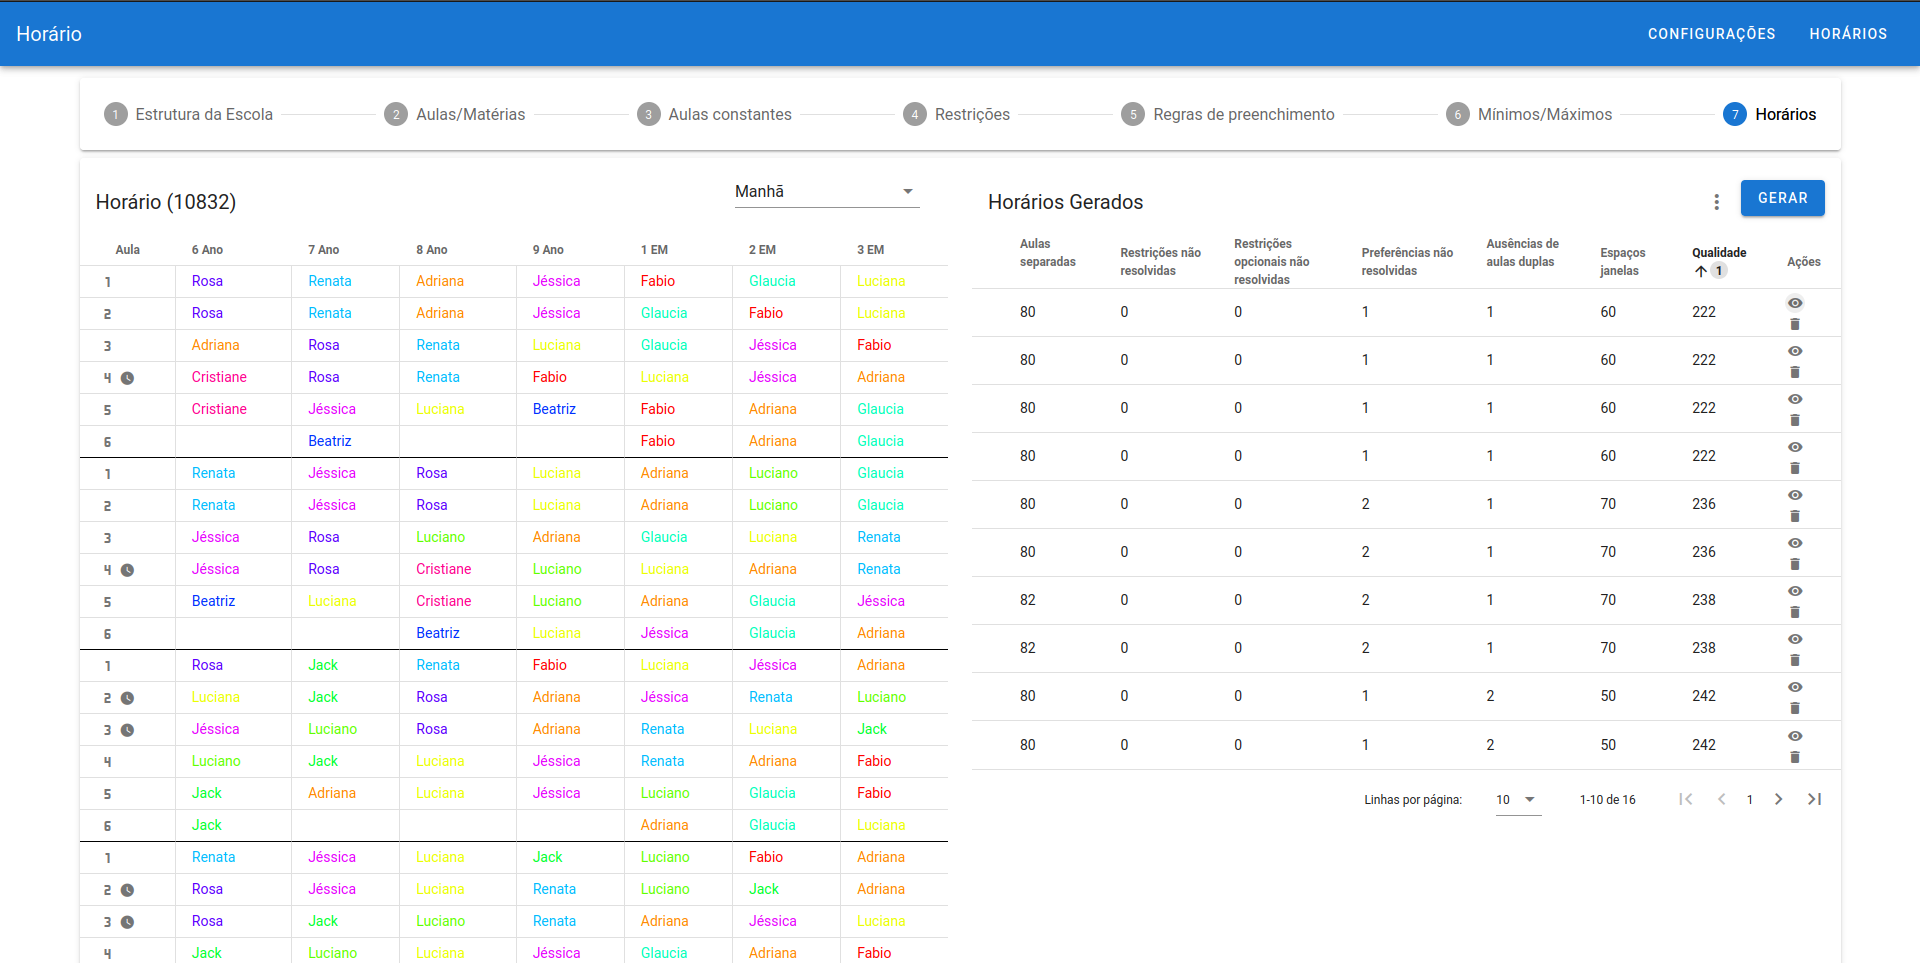
\includegraphics[width=0.8\textwidth]{./dados/figuras/tela_horarios}
	\fonte{Autor}
	\label{fig:tela-horarios}
\end{figure}
\newpage
\subsection{USUÁRIOS E AUTENTICAÇÃO}

Para controlar a visibilidade de informações no sistema desenvolvido, implementou-se um sistema de usuários. A melhoria consistiu na:

\begin{enumerate}
	\item Criação de tabela de usuários no banco de dados;
	\item Associação da tabela ``configuracao'' com a tabela de usuários, para que fosse possível armazenar o usuário responsável por cada configuração;
	\item Criação da tela de login na interface web;
	\item Criação das rotas de cadastro e \textit{login} no servidor
	\item Criação do \textit{middleware} de autenticação
	\item Criação do \textit{middleware} de validação da configuração
\end{enumerate}

\subsubsection{Adaptação do banco de dados}
A aplicação dos itens 1 e 2 foi realizada diretamente no banco de dados, através da criação da tabela mencionada e a chave estrangeira possibilitando a associação de cada usuário a múltiplas configurações. Após estas alterações, o diagrama entidade relacionamento do banco de dados passa a ser representado pela figura \ref{fig:er_atualizado}.

\begin{figure}[!htb]
	\centering
	\caption{Modelo Entidade-Relacionamento com adição da tabela de usuários}
	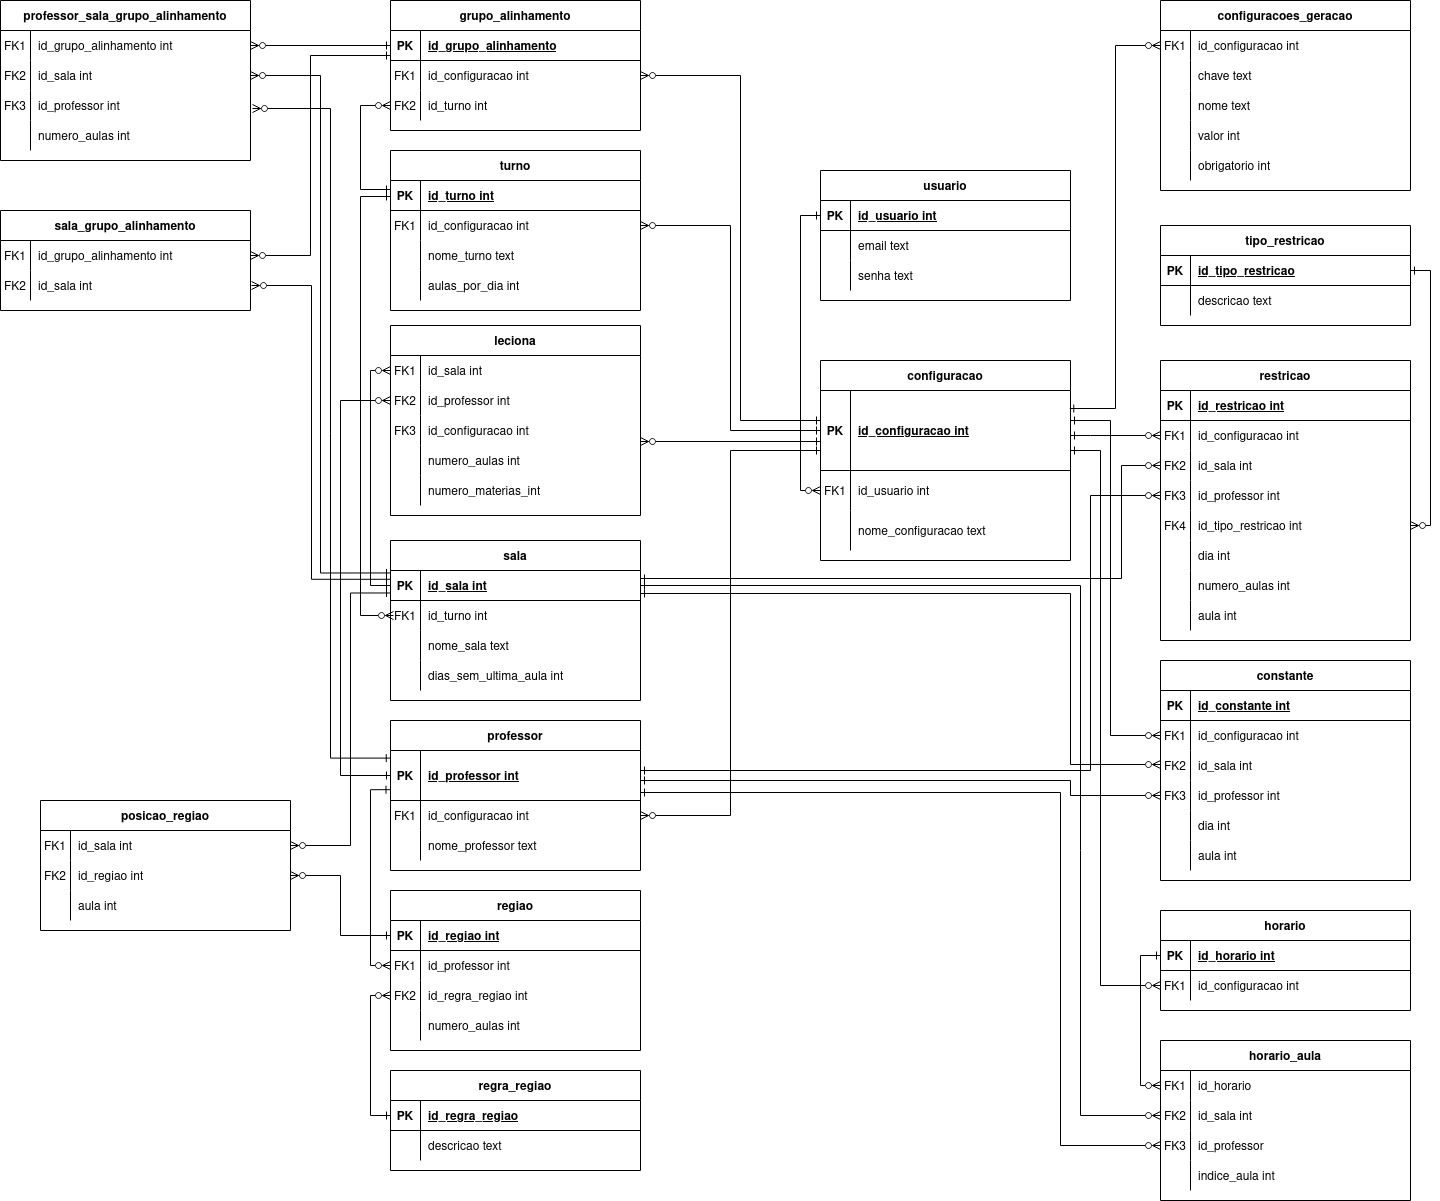
\includegraphics[width=0.65\textwidth]{./dados/figuras/er_horario_com_usuario}
	\fonte{Autor}
	\label{fig:er_atualizado}
\end{figure}

\subsubsection{Tela de login}
Como pode ser visto na figura \ref{fig:login}, desenvolveu-se uma tela simples de \textit{login}, a qual também desempenha a função de cadastro de novos usuários.

\begin{figure}[!htb]
	\centering
	\caption{Tela de Acesso}
	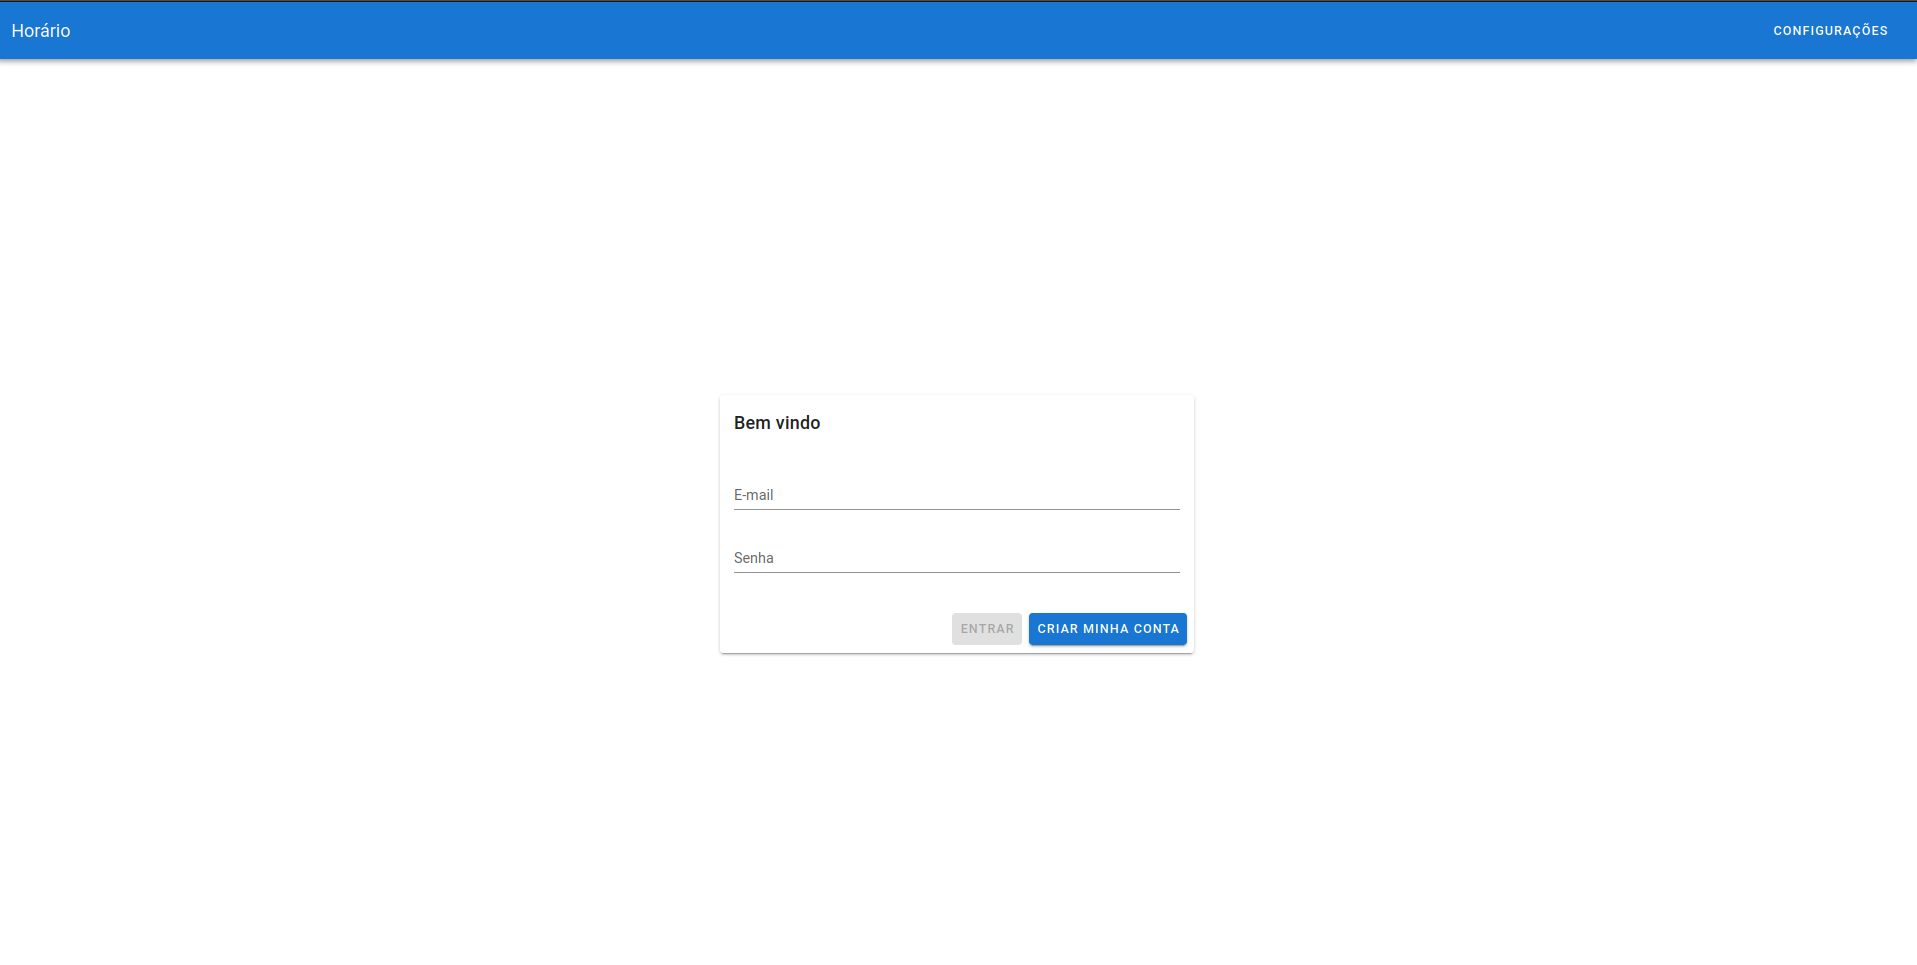
\includegraphics[width=1\textwidth]{./dados/figuras/telaLogin}
	\fonte{Autor}
	\label{fig:login}
\end{figure}
\pagebreak

\subsubsection{Rotas de autenticação}
Para a implementação das rotas de cadastro e \textit{login}, utilizou-se além do \textit{framework ExpressJS}, os pacotes JWT (\textit{Json Web Token}) e \textit{bcrypt}. O pacote JWT é utilizado para gerar \textit{tokens}, que são enviados para a interface web e podem ser utilizados para autenticar os usuários; já o \textit{bcrypt} é utilizado para gerar e validars as \textit{hashes} das senhas dos usuários, para que nunca sejam armazenadas senhas em texto pleno no banco de dados.

A função utilizada pela nova rota de cadastro pode vista na figura \ref{fig:metodoCadastro}. A função ``register'' realiza a validação dos parâmetros, e cria um usuário no banco de dados, caso já não exista outro com o mesmo e-mail. Além disso, a função retorna um \textit{token} JWT para a interface web, para que seja possível verificar a autenticidade das próximas requisições realizadas pelo usuário. 

\begin{figure}[!htb]
	\centering
	\caption{Método de Cadastro}
	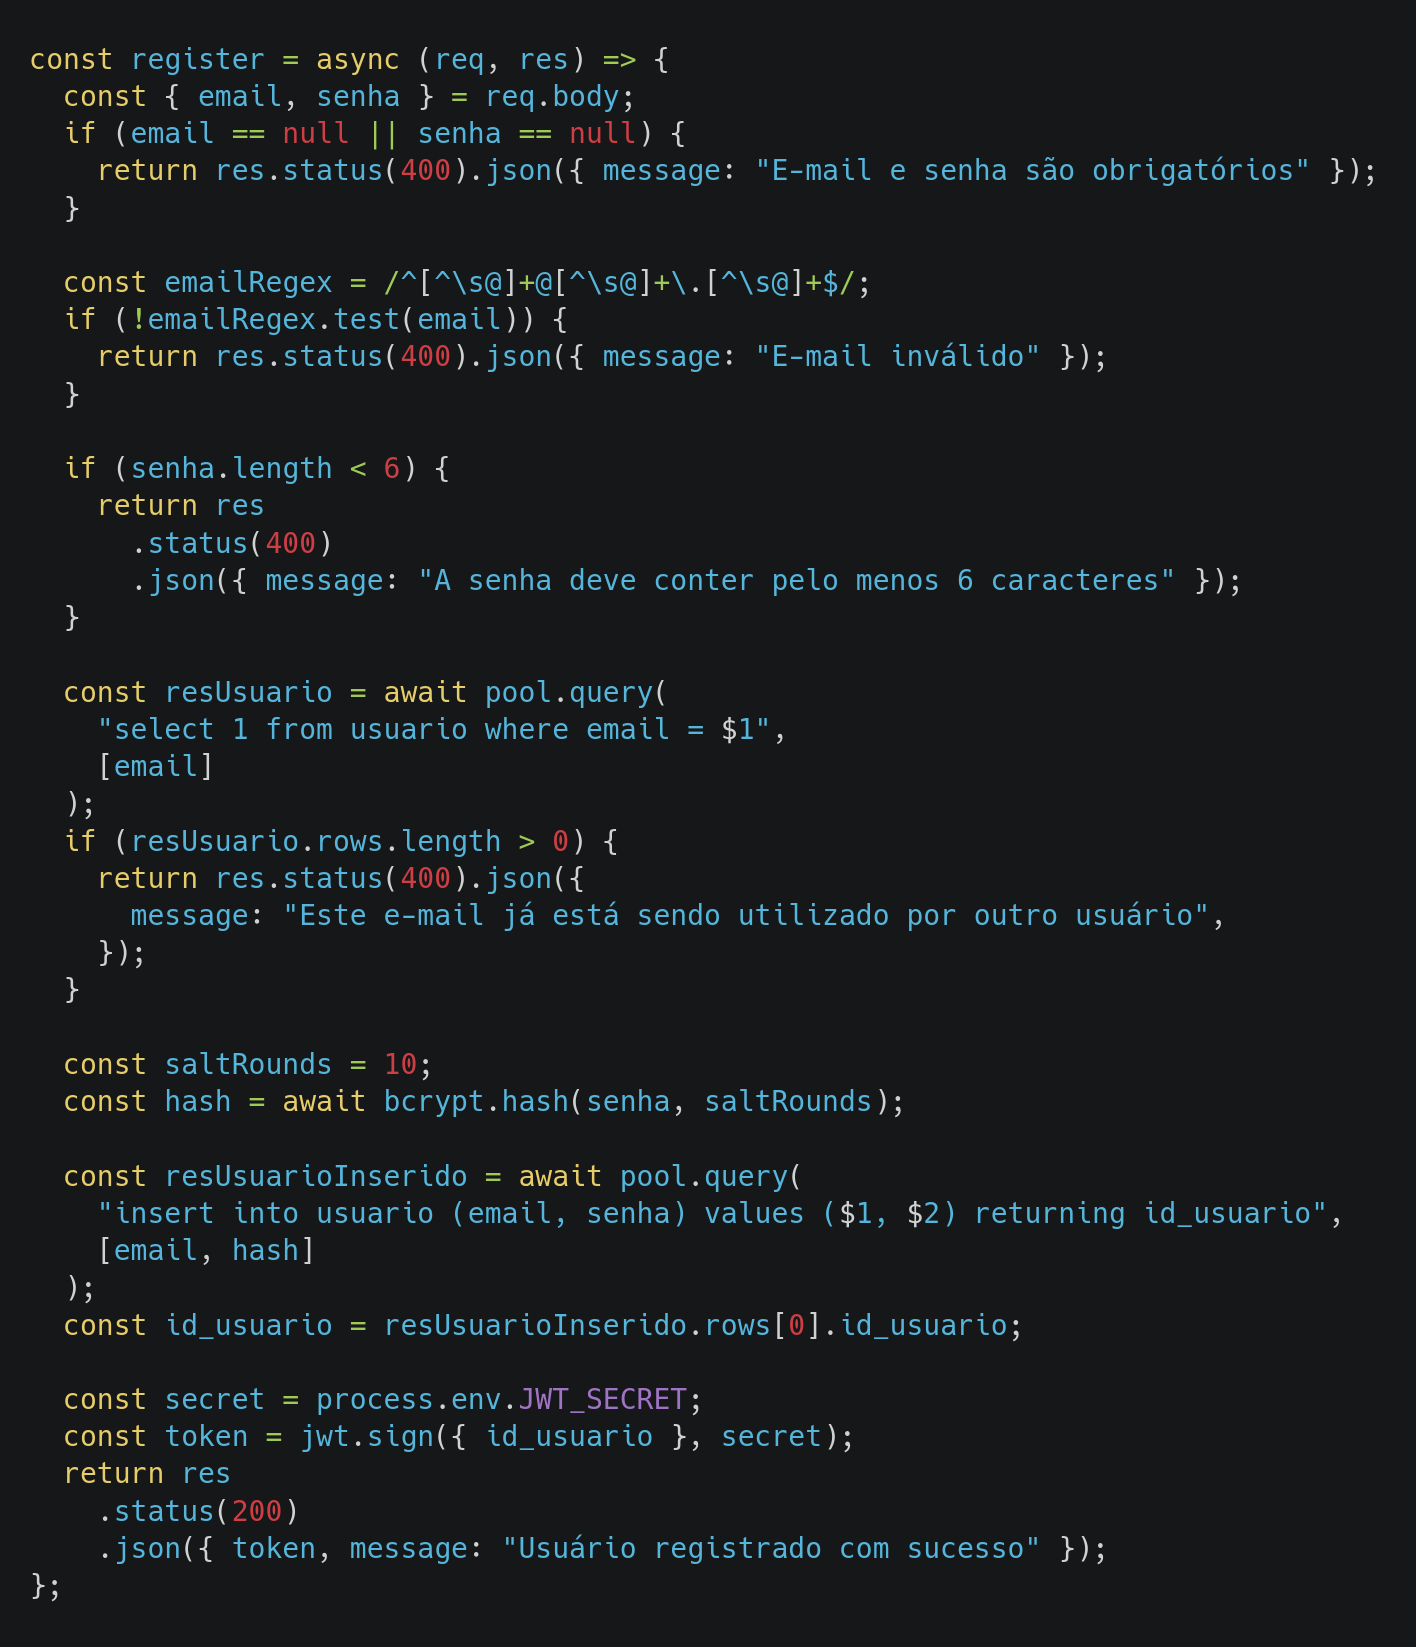
\includegraphics[width=0.8\textwidth]{./dados/figuras/register}
	\fonte{Autor}
	\label{fig:metodoCadastro}
\end{figure}
\pagebreak

A função de \textit{login}, visível na figura \ref{fig:metodoLogin} é similar, realizando validação dos parâmetros, autenticação do usuário através da comparação de senhas utilizando o pacote \textit{bcrypt} e geração de \textit{token} JWT. Vale citar que em ambas as rotas de autenticação, é inserido no \textit{payload} do \textit{token} o identificador do usuário, que posteriormente pode ser utilizado pelos \textit{middlewares} para a realização de validações.

\begin{figure}[!htb]
	\centering
	\caption{Método de Login}
	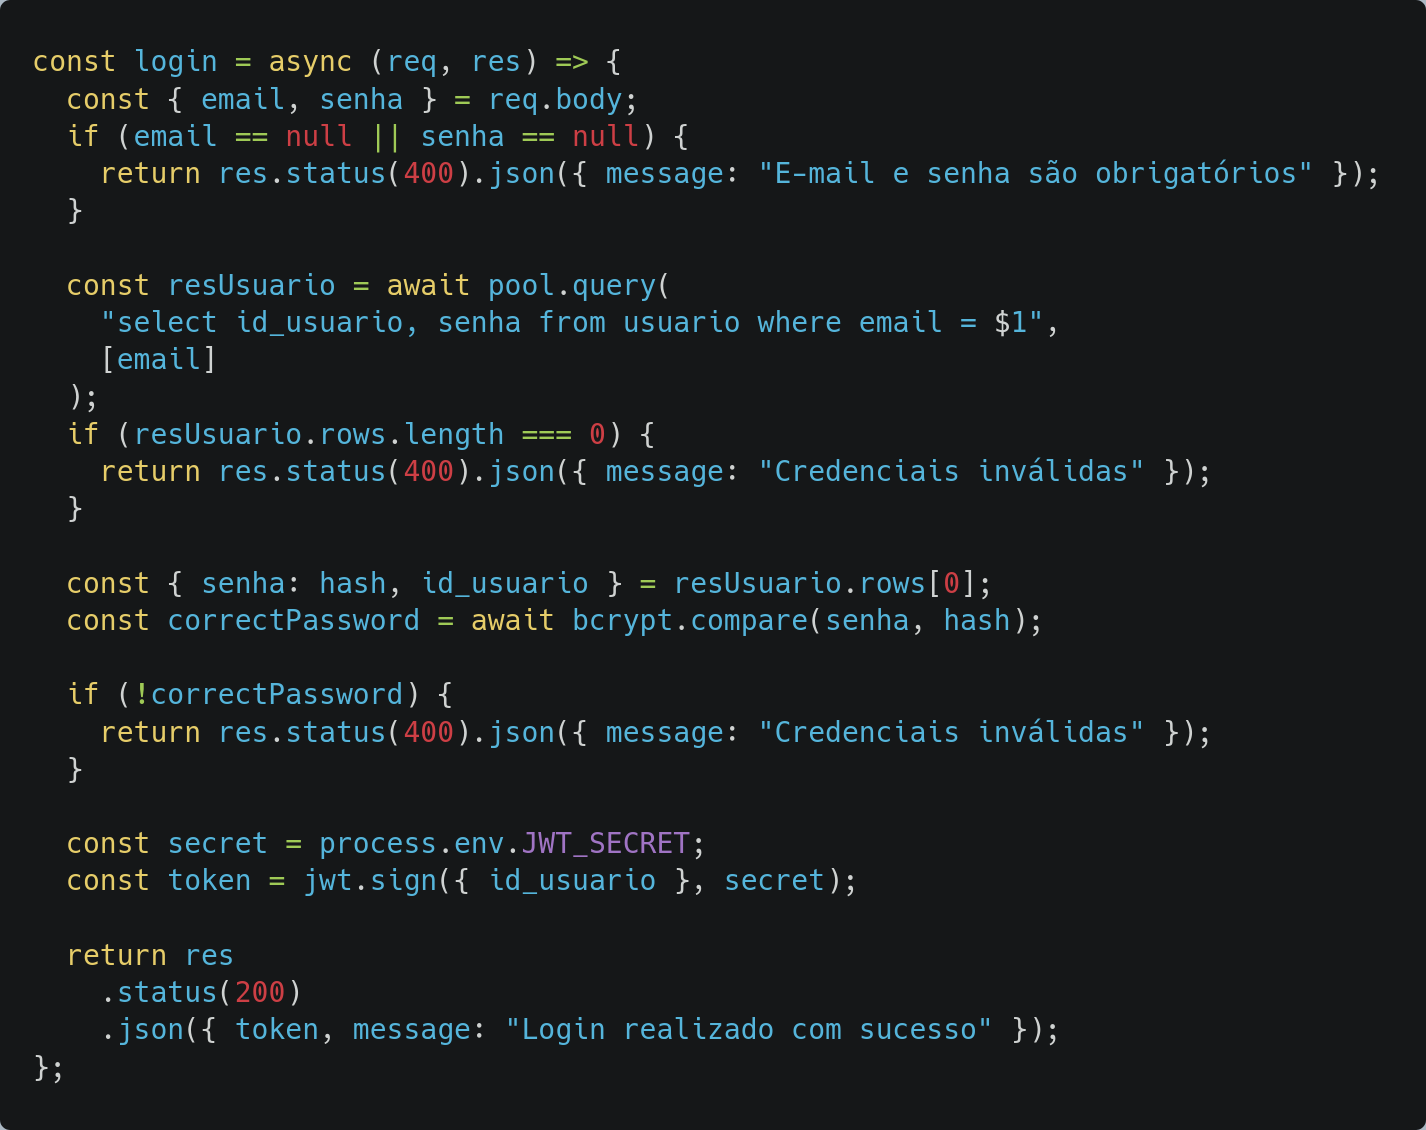
\includegraphics[width=0.8\textwidth]{./dados/figuras/login}
	\fonte{Autor}
	\label{fig:metodoLogin}
\end{figure}
\pagebreak

\subsubsection{Middlewares}
Foram criadas duas funções \textit{middleware} relacionadas aos usuários. A primeira é responsável por assegurar que apenas usuários propriamente autenticados tenham acesso aos recursos protegidos do sistema. Como pode ser visto na figura \ref{fig:auth}, essa verificação é realizada através da verificação da presença de um \textit{token} JWT válido no \textit{header ``authorization''} da requisição.

\begin{figure}[!htb]
	\centering
	\caption{Middleware de autenticação}
	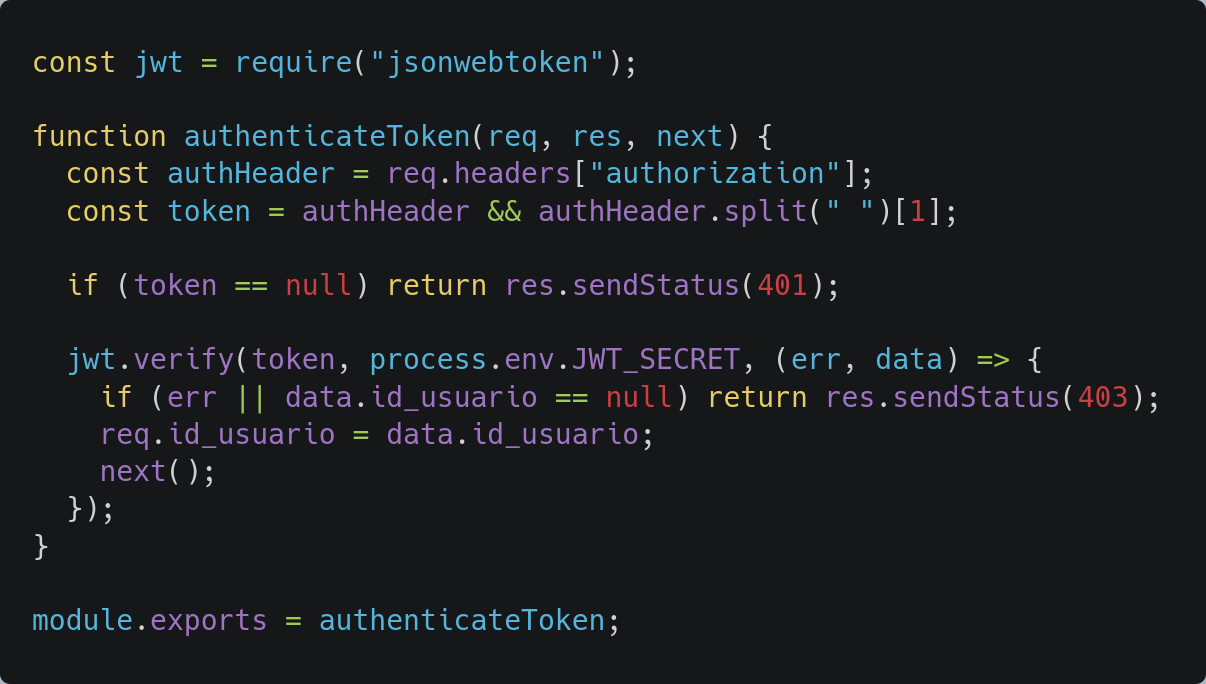
\includegraphics[width=0.8\textwidth]{./dados/figuras/authMiddleware}
	\fonte{Autor}
	\label{fig:auth}
\end{figure}
\pagebreak

O outro middleware criado tem como objetivo assegurar que um usuário possa consultar apenas as configurações pelas quais seja responsável. Isso é feito utilizando o identificador do usuário, presente no \textit{payload} do \textit{token} JWT, conforme a figura \ref{fig:configMiddleware}. Caso o usuário não tenha um vínculo com a configuração que está tentando acessar, a requisição é bloqueada.

\begin{figure}[!htb]
	\centering
	\caption{Middleware de validação da configuração}
	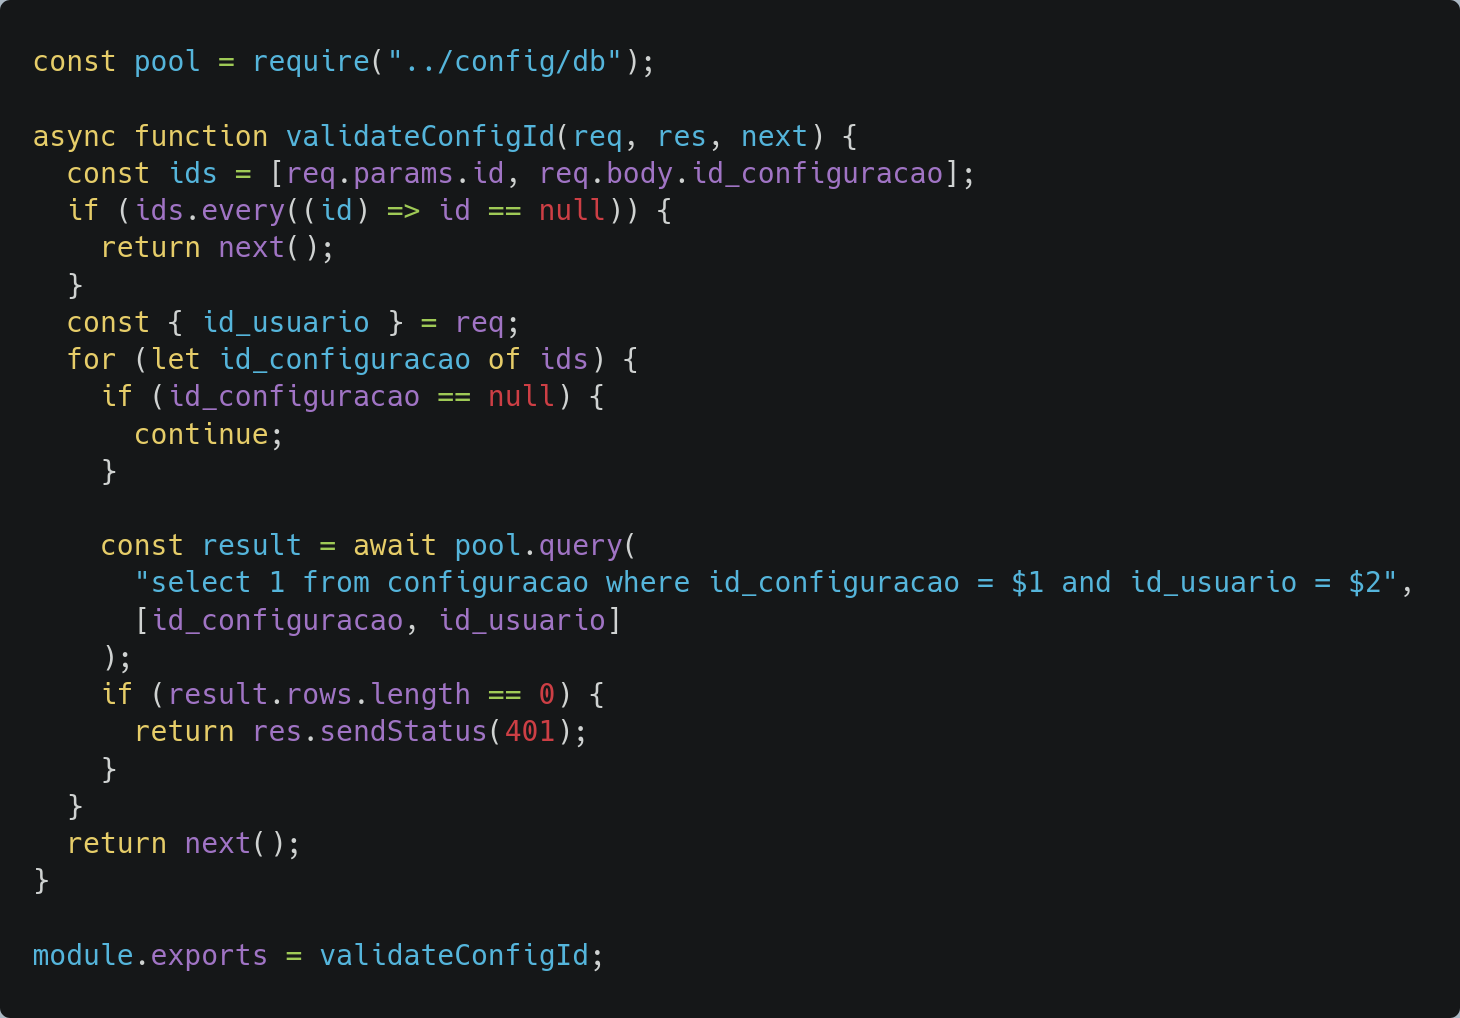
\includegraphics[width=0.8\textwidth]{./dados/figuras/configMiddleware}
	\fonte{Autor}
	\label{fig:configMiddleware}
\end{figure}
\pagebreak



\subsection{ALOCAÇÃO DE MATÉRIAS}

Durante os incrementos anterioriores, o otimizador gerava grades horárias que continham apenas os nomes dos professores alocados para aula. Em outras palavras, as grades eram matrizes nas quais as linhas eram os horários disponíveis, as colunas eram as salas e cada posição na matriz representava qual professor deveria ministrar a aula naquele horário.

A alocação dos professores é muito importante para a resolução do problema, pois apresenta a maior parte das retrições e dificuldades relacionadas, como os conflitos, por exemplo. Entretando, em termos de completude, as grades horárias devem ter também a alocação de matérias em cada horário de aula, visto que cada professor pode ministrar aulas de mais de uma matéria. As alterações necessárias para possibilitar isso foram:

\begin{enumerate}
	\item Alterar a modelagem do banco de dados para comportar informações relacionadas às matérias;
	\item Alterar telas da interface web para que fosse possível configurar as matérias;
	\item Alterar rotas do servidor para persistir as matérias;
	\item Alterar código do otimizador para produzir grades horárias com matérias
\end{enumerate}

\subsubsection{Alteração no banco de dados}
Para armazenar informações relacionadas às matérias, a modelagem do banco de dados foi alterada com a criação de três tabelas: 
\begin{itemize}
	\item materia
	\item horario-materias: representa uma grade horária de matérias, que tem vínculo com a entidade principal da grade horária
	\item horario-materia: representa uma matéria alocada em determinada posição de uma grade horária
\end{itemize}

Com esta modelagem atualizada, presente na figura \ref{fig:modelagemMateiras}, cada grade horária de professores, pode ter diferentes opções de grades de matérias.

\begin{figure}[!htb]
	\centering
	\caption{Modelo Entidade-Relacionamento com Matérias}
	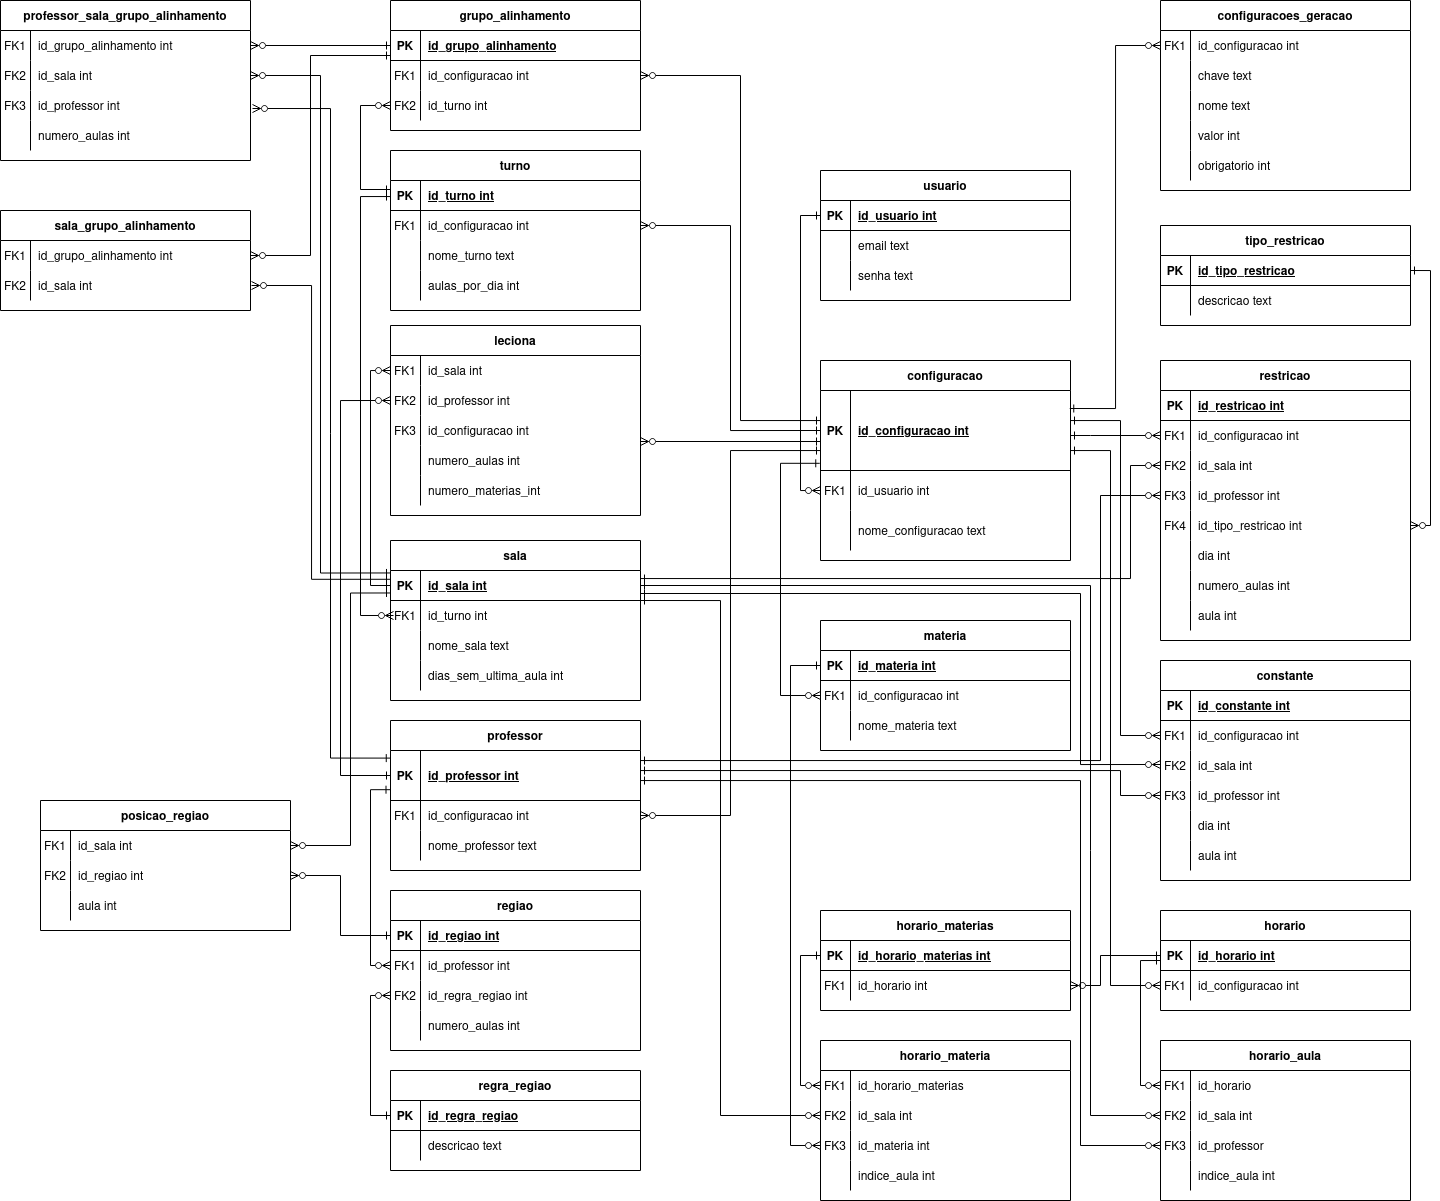
\includegraphics[width=0.65\textwidth]{./dados/figuras/er_materias}
	\fonte{Autor}
	\label{fig:modelagemMateiras}
\end{figure}
\pagebreak

\subsubsection{Alteração de telas}
Com a adição do conceito das matérias ao sistema, algumas telas da interface precisaram ser modificadas. A primeira destas, foi a tela inicial da configuração, ou seja, a tela de "Estrutura da Escola", cuja alteração pode ser vista na figura \ref{fig:estruturaAtualizada} consistiu na adição de uma seção para cadastro e visualização de matérias, semelhante ao componente de cadastro de professores.

\begin{figure}[!htb]
	\centering
	\caption{Estrutura da Escola com Matérias}
	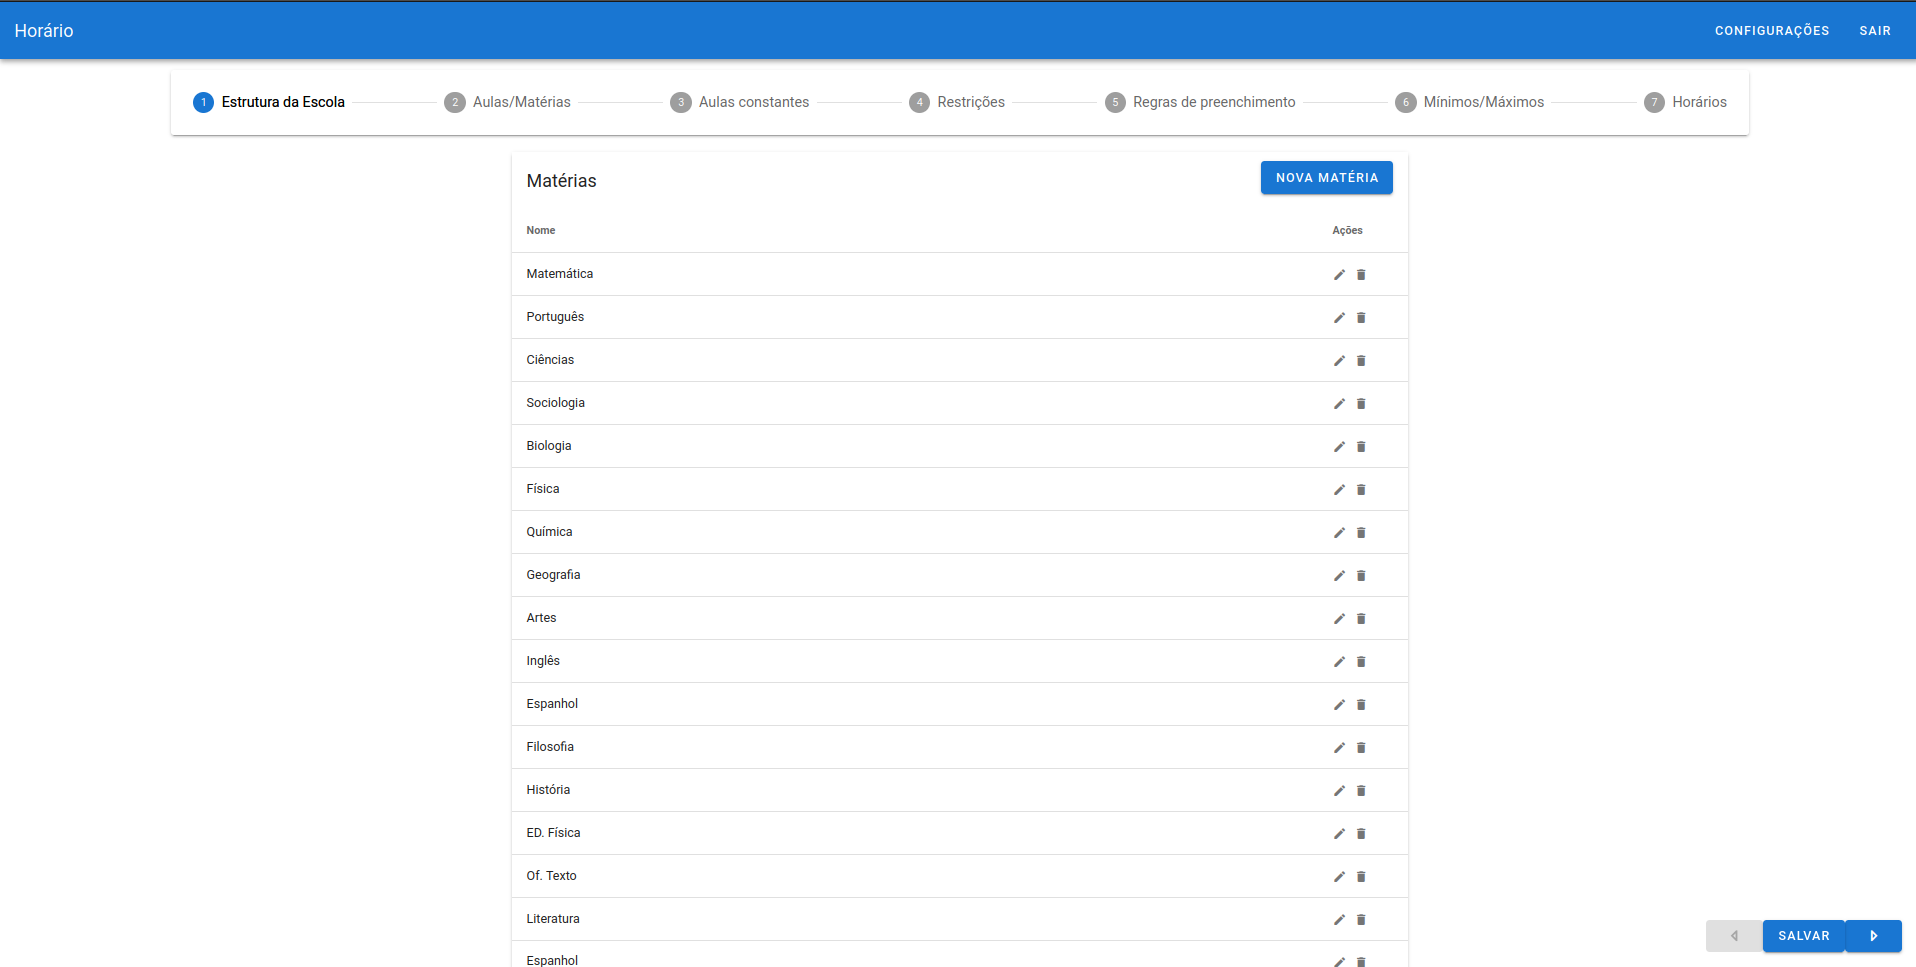
\includegraphics[width=0.65\textwidth]{./dados/figuras/alteracaoEstrutura}
	\fonte{Autor}
	\label{fig:estruturaAtualizada}
\end{figure}
\pagebreak

Além da tela de estrutura, a segunda aba da configuração ("Aulas/Matérias") foi alterada para que fosse possível vincular matérias aos professores, e configurar a quantidade de aulas de cada matéria deve ser ministrada semanalmente, conforme a figura \ref{fig:alteracaoAulas}.

\begin{figure}[!htb]
	\centering
	\caption{Tela de configuração de quantidades de aulas por matéria}
	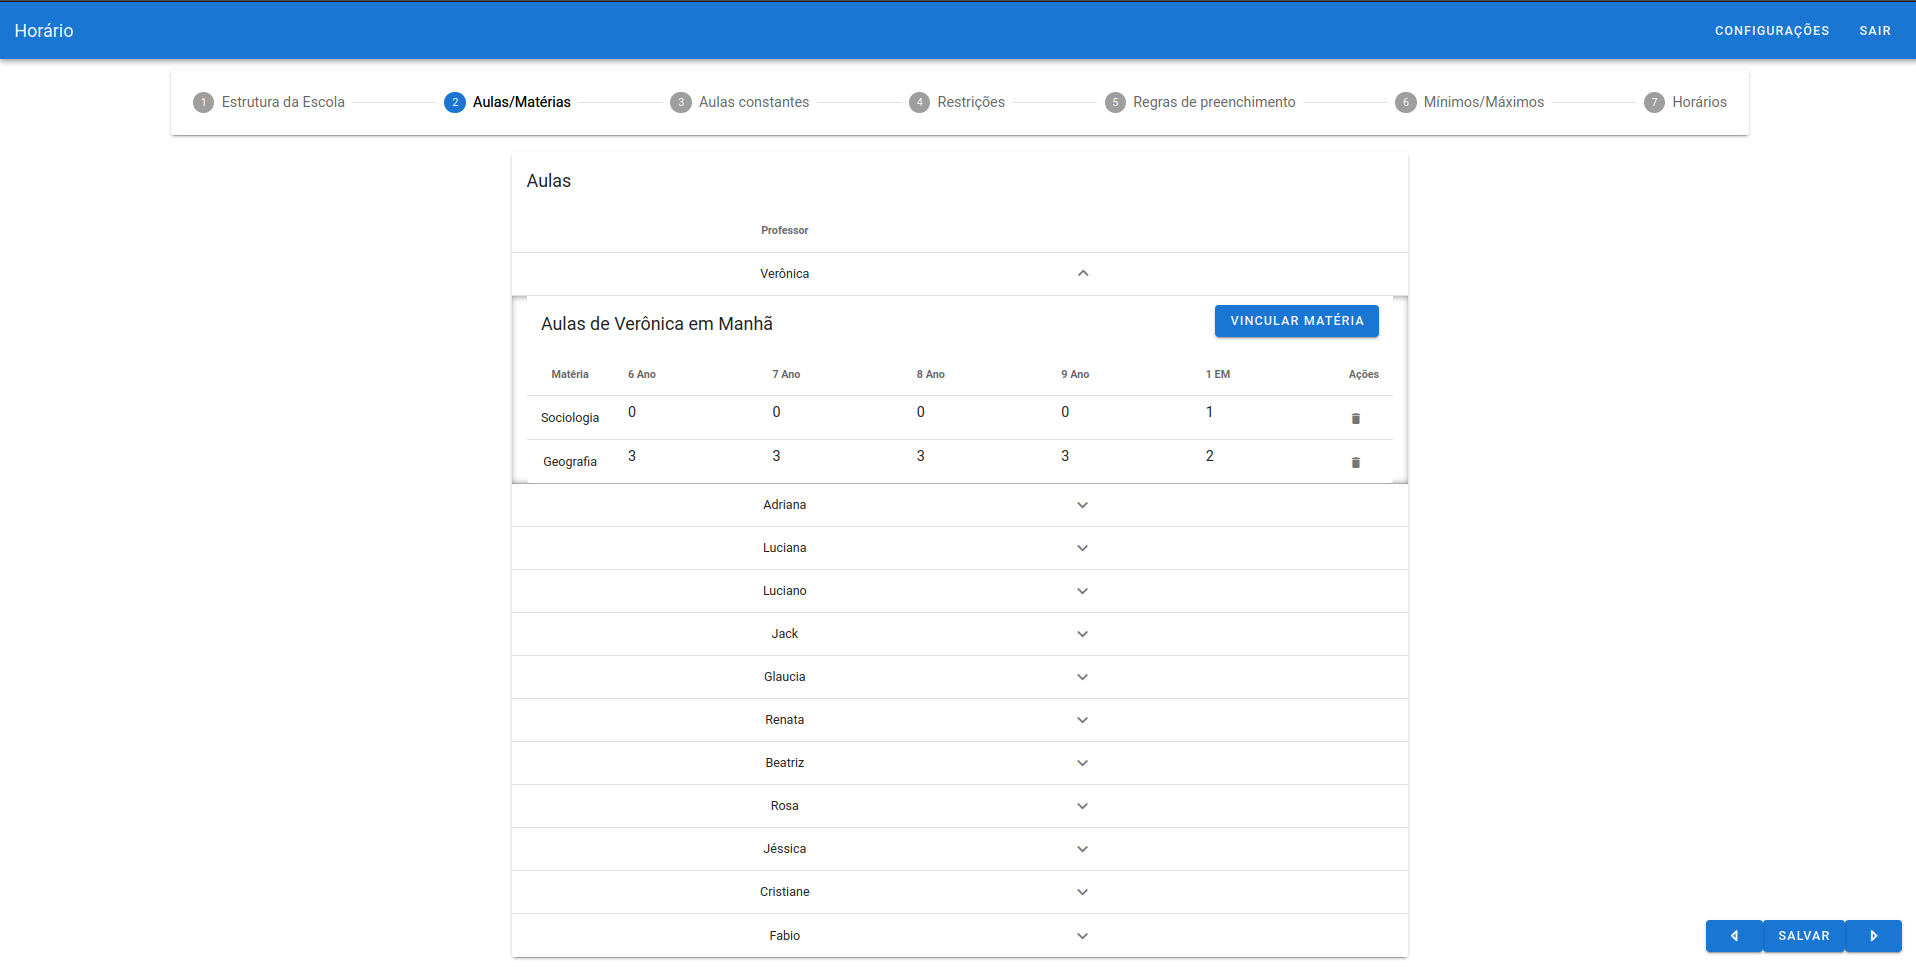
\includegraphics[width=0.65\textwidth]{./dados/figuras/alteracaoAulas}
	\fonte{Autor}
	\label{fig:alteracaoAulas}
\end{figure}

Por fim, na tela final da configuração, representável por exibir as grades horárias geradas, foi necessário alterar o componente da grade para incluir, além dos nomes dos professores, os nomes das matérias alocadas para cada horário, como pode ser visto na figura \ref{fig:alteracaoHorario}.

\begin{figure}[!htb]
	\centering
	\caption{Visualização de grade horária com matérias}
	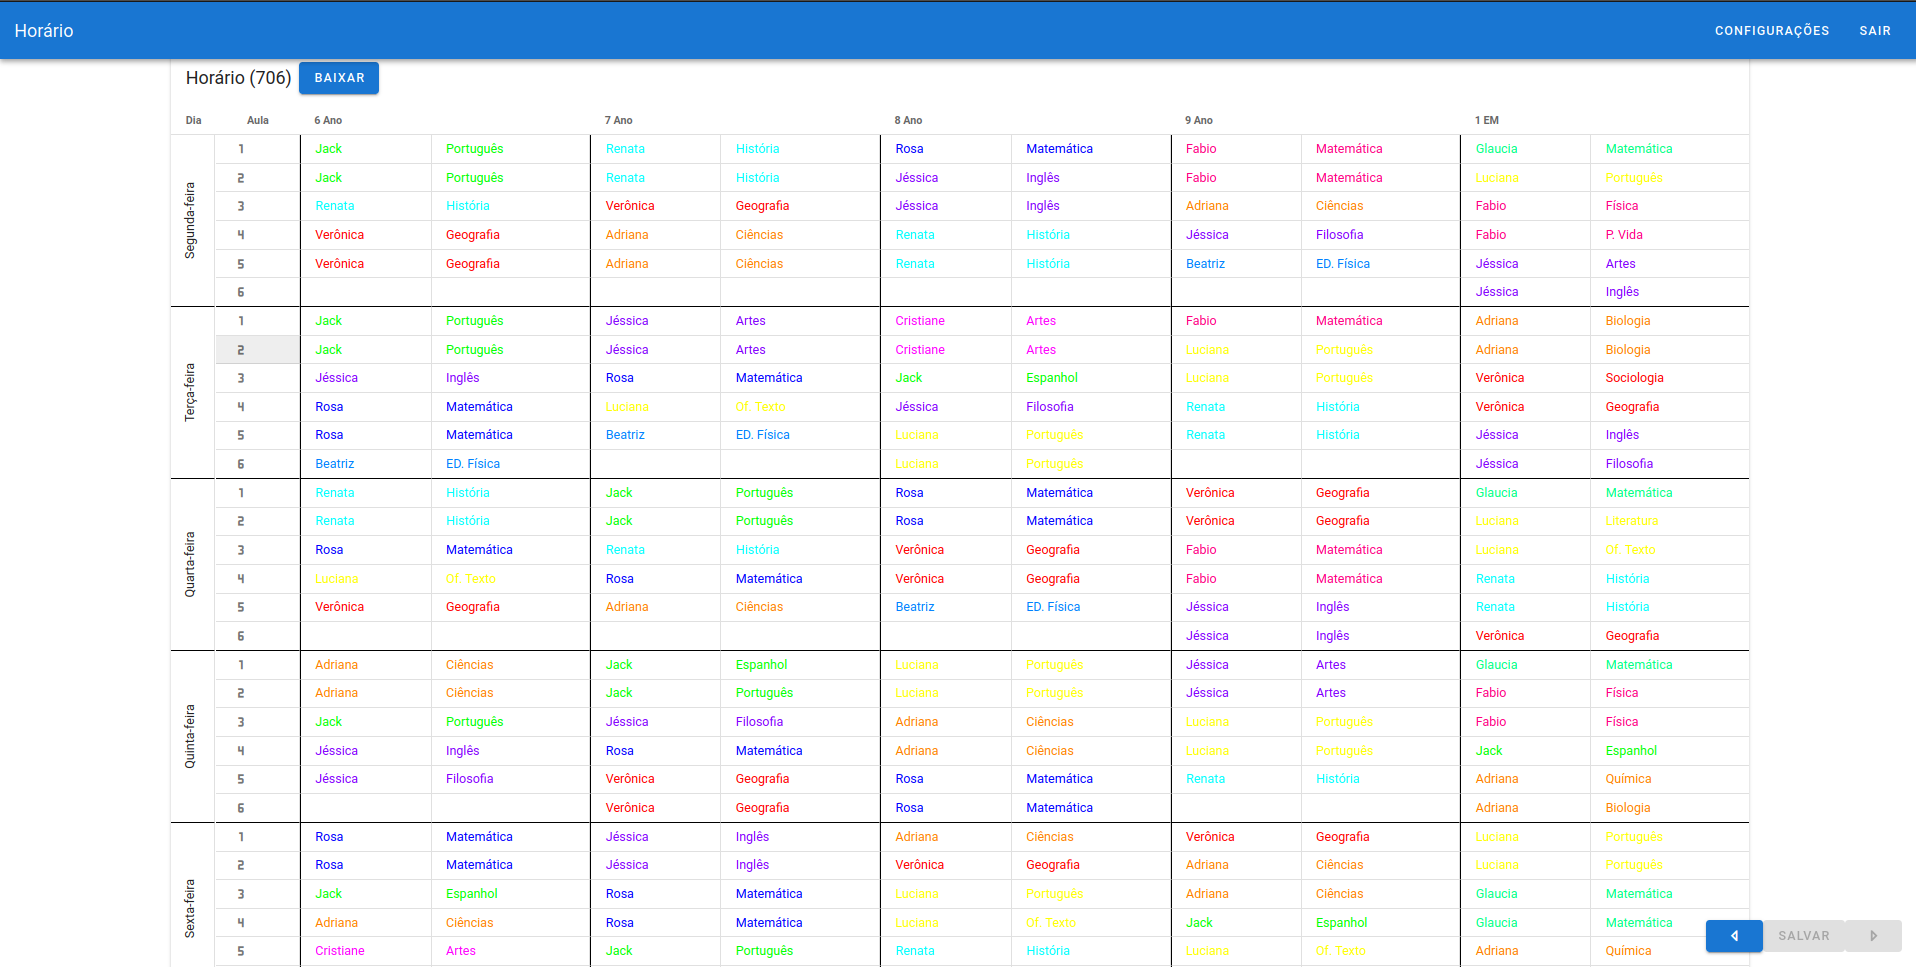
\includegraphics[width=0.65\textwidth]{./dados/figuras/alteracaoHorarios}
	\fonte{Autor}
	\label{fig:alteracaoHorario}
\end{figure}

\subsubsection{Alteração de métodos no servidor}
A adição das matérias também envolveu algumas alterações no servidor. As rotas alteradas para acomodar a melhoria foram rotas de armazenamento e consulta da estrutura da escola, aulas e grades horárias.

Evidentemente, as funções responsáveis por essas rotas precisaram ser modificadas para interagir corretamente com as novas tabelas criadas durante o desenvolvimento deste incremento.

\subsubsection{Matérias no otimizador}
Após as alterações na interface, servidor e banco de dados, o sistema estava pronto para lidar com as informações relacionadas às matérias, faltando apenas a incorporação destas na geração de grades horárias por parte do otimizador. Para realizar isso, implementou-se um método análogo ao \autoref{alg:otimizadorComRestricoes}, porém voltado à geração de grades de matérias.

A diferença é que o novo método implementado obtém determinada grade horária gerada pelo \autoref{alg:otimizadorComRestricoes}, e realiza as operações necessárias para preencher a grade com matérias. Vale ressaltar que essas operações são semelhantes à geração da grade de aulas dos professores: preenchimento da grade inicial, cálculo da variação de custo, realização de trocas de posições e armazenamento das soluções.

O método de geração de grades foi aplicado no otimizador de forma que cada vez que uma grade horária de professores é salva no banco de dados, esta também já tem a sua grade horária de matérias gerada, completando assim o processo de otimização da grade, conforme o \autoref{alg:otimizadorCompleto}.

\begin{algorithm}
	\caption{Otimizador com matérias}
	\label{alg:otimizadorCompleto}
	\KwIn{Lista de professores $LP$, lista de turmas $LT$, matriz de aulas e matérias por professor por turma $MA$, temperatura inicial $TI$, Taxa de resfriamento $TR$}
	\KwOut{Grade horária de matérias e professores otimizada}
	$temperatura \leftarrow TI$\\
	$grade \leftarrow$ CriaGradeInicial$(LP, LT, MA)$\\
	$iteracoesSemAlteracao \leftarrow 0$\\
	$solucoes \leftarrow$ lista vazia\\
	\While {condição de parada não atingida} {
		$deltaTotal \leftarrow 0$\\
		\For {$passo = 0$ até $numeroPassos$} {
			$turma \leftarrow grade.EscolheTurmaAleatoria()$\\
			$linhas \leftarrow grade.EscolheHorariosAleatoriosValidos(sala)$\\
			$delta \leftarrow grade.CalculaDelta(sala, linhas)$\\
			$probabilidade \leftarrow e^{-delta/temperatura}$\\
			$valorAceite \leftarrow Aleatorio(0, 1)$\\
			\If {$delta < 0$ ou $probabilidade \ge valorAceite$} {
				$grade.PermutaProfessores(sala, linha1, linha2)$\\
				$deltaTotal \leftarrow deltaTotal + delta$\\
				\If {grade não existe na lista de soluções} {
					insere grade na lista de soluções\\
					limita lista de soluções às 100 melhores grades\\
				}
			}
		}
		\eIf {$delta = 0$} {
			$iteracoesSemAlteracao \leftarrow iteracoesSemAlteracao + 1$\\
		}{
			$iteracoesSemAlteracao \leftarrow 0$\\
		}
		\If {$iteracoesSemAlteracao \ge 15$} {
			\For{gradeProfessores em EscolherGradesRelevantes(solucoes)} {
				SalvaGradeProfessores$(gradeProfessores)$\\
				$gradesMaterias \leftarrow$ GeraGradesMaterias$(gradeProfessores)$\\
				SalvarMelhorGradeMaterias$(gradesMaterias)$\\
			}
			apaga lista de soluções\\
			$temperatura \leftarrow TI$\\
			$iteracoesSemAlteracao \leftarrow 0$\\
		}
		$temperatura \leftarrow temperatura * TR$
	}
\end{algorithm}

\subsection{VALIDAÇÃO DE CONFIGURAÇÕES}

Devido à grade quantidade de configurações necessárias para parametrizar a geração de uma grade horária, erros de configurações por parte dos usuários são inevitáveis. Tendo isto em mente, implementou-se uma seção de cótigo no otimizador, responsável pela validação das informações providenciadas pelo usuário.

Vale ressaltar que esta validação não garante que é possível gerar uma grade horária de acordo com as configurações providas, mas ela deve evitar alguns dos erros mais comuns. As validações realizadas foram:

\begin{enumerate}
	\item O total de aulas configurado para cada sala deve ser correto, de acordo com o número de dias da grade horária e quantidade de aulas por dia;
	\item Para cada sala, nenhum professor pode ter mais aulas agendadas do que a sala acomoda;
	\item Nenhum professor pode ter mais aulas constantes configuradas do que o seu total de aulas naquela sala;
	\item Não pode haver uma restrição e aula constante para determinado professor na mesma posição da grade horária;
\end{enumerate}

Estas validações são executadas antes do início das otimizações das grades horárias, e caso haja algum erro de configuração, é exibida uma mensagem alertando o usuário, conforme a \autoref{fig:erroValidacao}.

\begin{figure}[!htb]
	\centering
	\caption{Mensagem de erro de validação}
	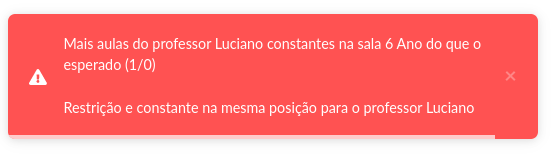
\includegraphics[width=1\textwidth]{./dados/figuras/erroValidacao}
	\fonte{Autor}
	\label{fig:erroValidacao}
\end{figure}
\pagebreak

\section{EXPORTAÇÃO DE GRADES HORÁRIAS}